\section{Kết quả thực nghiệm và nhận xét}

\subsection{Kết quả thực nghiệm}

\subsubsection{Đầu vào có thứ tự ngẫu nhiên}

\begin{table}[H] % Use [H] to force the table to be placed here
    \centering
    \caption{Kết quả thực nghiệm với đầu vào có thứ tự ngẫu nhiên (Nhóm 1)}
    \begin{tblr}{
      column{even} = {r},
      column{3} = {r},
      column{5} = {r},
      column{7} = {r},
      cell{1}{2} = {c=2}{c},
      cell{1}{4} = {c=2}{c},
      cell{1}{6} = {c=2}{c},
      cell{2}{2} = {c},
      cell{2}{3} = {c},
      cell{2}{4} = {c},
      cell{2}{5} = {c},
      cell{2}{6} = {c},
      cell{2}{7} = {c},
      hline{1,3,14} = {-}{},
      hline{2} = {2-7}{},
    }
        \textbf{Data size} & \textbf{10,000} &                      & \textbf{30,000} &                      & \textbf{50,000} &                      \\
        \textbf{Metrics}   & \textbf{Time}   & \textbf{Comparisons} & \textbf{Time}   & \textbf{Comparisons} & \textbf{Time}   & \textbf{Comparisons} \\
        Selection Sort     & 110             & 100009999            & 870             & 900029999            & 2474            & 2500049999           \\
        Insertion Sort     & 58              & 49852722             & 504             & 450424387            & 1481            & 1244875082           \\
        Shell Sort         & 271             & 100009999            & 2692            & 900029999            & 7542            & 2500049999           \\
        Bubble Sort        & 268             & 100009999            & 2639            & 900029999            & 7491            & 2500049999           \\
        Heap Sort          & 1               & 638425               & 6               & 2150786              & 10              & 3771772              \\
        Merge Sort         & 3               & 583832               & 9               & 1937240              & 15              & 3383319              \\
        Quick Sort         & 1               & 276045               & 5               & 916849               & 6               & 1636700              \\
        Radix Sort         & 0               & 140056               & 1               & 510070               & 2               & 850070               \\
        Counting Sort      & 0               & 80000                & 0               & 240000               & 0               & 382769               \\
        Shaker Sort        & 219             & 75877345             & 1986            & 678034901            & 5519            & 1868558231           \\
        Flash Sort         & 0               & 97658                & 0               & 285201               & 1               & 451390
    \end{tblr}
\end{table}

\begin{table}[H] % Use [H] to force the table to be placed here
    \centering
    \caption{Kết quả thực nghiệm với đầu vào có thứ tự ngẫu nhiên (Nhóm 2)}
    \begin{tblr}{
      column{even} = {r},
      column{3} = {r},
      column{5} = {r},
      column{7} = {r},
      cell{1}{2} = {c=2}{c},
      cell{1}{4} = {c=2}{c},
      cell{1}{6} = {c=2}{c},
      cell{2}{2} = {c},
      cell{2}{3} = {c},
      cell{2}{4} = {c},
      cell{2}{5} = {c},
      cell{2}{6} = {c},
      cell{2}{7} = {c},
      hline{1,3,14} = {-}{},
      hline{2} = {2-7}{},
    }
        \textbf{Data size} & \textbf{100,000} &                      & \textbf{300,000} &                      & \textbf{500,000} &                      \\
        \textbf{Metrics}   & \textbf{Time}    & \textbf{Comparisons} & \textbf{Time}    & \textbf{Comparisons} & \textbf{Time}    & \textbf{Comparisons} \\
        Selection Sort     & 10378            & 10000099999          & 91156            & 90000299999          & 306006           & 250000499999         \\
        Insertion Sort     & 5879             & 5026592949           & 68865            & 44937080911          & 231821           & 125044404674         \\
        Shell Sort         & 30370            & 10000099999          & 396729           & 90000299999          & 1182221          & 250000499999         \\
        Bubble Sort        & 31385            & 10000099999          & 454882           & 90000299999          & 1203413          & 250000499999         \\
        Heap Sort          & 21               & 8044992              & 79               & 26487787             & 140              & 45972193             \\
        Merge Sort         & 31               & 7166010              & 103              & 23383601             & 180              & 40383061             \\
        Quick Sort         & 11               & 3341712              & 54               & 10434674             & 112              & 18476753             \\
        Radix Sort         & 4                & 1700070              & 16               & 5100070              & 25               & 8500070              \\
        Counting Sort      & 1                & 732769               & 3                & 2132769              & 6                & 3532769              \\
        Shaker Sort        & 24340            & 7519014091           & 323182           & 67598742089          & 1018829          & 187569730819         \\
        Flash Sort         & 2                & 905677               & 7                & 2611012              & 19               & 4335083
    \end{tblr}
\end{table}

\subsubsection{Đầu vào có thứ tự gần được sắp xếp}

\begin{table}[H] % Use [H] to force the table to be placed here
    \centering
    \caption{Kết quả thực nghiệm với đầu vào có thứ tự gần được sắp xếp (Nhóm 1)}
    \begin{tblr}{
      column{even} = {r},
      column{3} = {r},
      column{5} = {r},
      column{7} = {r},
      cell{1}{2} = {c=2}{c},
      cell{1}{4} = {c=2}{c},
      cell{1}{6} = {c=2}{c},
      cell{2}{2} = {c},
      cell{2}{3} = {c},
      cell{2}{4} = {c},
      cell{2}{5} = {c},
      cell{2}{6} = {c},
      cell{2}{7} = {c},
      hline{1,3,14} = {-}{},
      hline{2} = {2-7}{},
    }
        \textbf{Data size} & \textbf{10,000} &                      & \textbf{30,000} &                      & \textbf{50,000} &                      \\
        \textbf{Metrics}   & \textbf{Time}   & \textbf{Comparisons} & \textbf{Time}   & \textbf{Comparisons} & \textbf{Time}   & \textbf{Comparisons} \\
        Selection Sort     & 106             & 100009999            & 868             & 900029999            & 2472            & 2500049999           \\
        Insertion Sort     & 0               & 129726               & 1               & 486366               & 1               & 560354               \\
        Shell Sort         & 96              & 100009999            & 812             & 900029999            & 2290            & 2500049999           \\
        Bubble Sort        & 94              & 100009999            & 828             & 900029999            & 2259            & 2500049999           \\
        Heap Sort          & 2               & 669904               & 5               & 2236774              & 9               & 3925280              \\
        Merge Sort         & 3               & 503802               & 7               & 1637853              & 12              & 2845326              \\
        Quick Sort         & 0               & 154995               & 1               & 501973               & 2               & 913890               \\
        Radix Sort         & 0               & 140056               & 1               & 510070               & 2               & 850070               \\
        Counting Sort      & 0               & 80001                & 0               & 240001               & 0               & 400001               \\
        Shaker Sort        & 1               & 299791               & 1               & 899791               & 2               & 1299845              \\
        Flash Sort         & 0               & 118969               & 0               & 356969               & 1               & 594969
    \end{tblr}
\end{table}

\begin{table}[H] % Use [H] to force the table to be placed here
    \centering
    \caption{Kết quả thực nghiệm với đầu vào có thứ tự gần được sắp xếp (Nhóm 2)}
    \begin{tblr}{
      column{even} = {r},
      column{3} = {r},
      column{5} = {r},
      column{7} = {r},
      cell{1}{2} = {c=2}{c},
      cell{1}{4} = {c=2}{c},
      cell{1}{6} = {c=2}{c},
      cell{2}{2} = {c},
      cell{2}{3} = {c},
      cell{2}{4} = {c},
      cell{2}{5} = {c},
      cell{2}{6} = {c},
      cell{2}{7} = {c},
      hline{1,3,14} = {-}{},
      hline{2} = {2-7}{},
    }
        \textbf{Data size} & \textbf{100,000} &                      & \textbf{300,000} &                      & \textbf{500,000} &                      \\
        \textbf{Metrics}   & \textbf{Time}    & \textbf{Comparisons} & \textbf{Time}    & \textbf{Comparisons} & \textbf{Time}    & \textbf{Comparisons} \\
        Selection Sort     & 11396            & 10000099999          & 137957           & 90000299999          & 1295243          & 250000499999         \\
        Insertion Sort     & 1                & 706102               & 2                & 1188582              & 2                & 1905186              \\
        Shell Sort         & 9538             & 10000099999          & 166585           & 90000299999          & 1319995          & 250000499999         \\
        Bubble Sort        & 9164             & 10000099999          & 135698           & 90000299999          & 1486996          & 250000499999         \\
        Heap Sort          & 17               & 8364715              & 57               & 27413296             & 104              & 47405047             \\
        Merge Sort         & 23               & 5851166              & 95               & 18733795             & 130              & 32137705             \\
        Quick Sort         & 5                & 1927723              & 13               & 6058264              & 28               & 10310769             \\
        Radix Sort         & 4                & 1700070              & 19               & 6000084              & 26               & 10000084             \\
        Counting Sort      & 1                & 800001               & 4                & 2400001              & 6                & 4000001              \\
        Shaker Sort        & 4                & 2999791              & 7                & 6599891              & 14               & 12999845             \\
        Flash Sort         & 2                & 1189967              & 6                & 3569970              & 13               & 5949970
    \end{tblr}
\end{table}

\subsubsection{Đầu vào có thứ tự đã được sắp xếp}

\begin{table}[H] % Use [H] to force the table to be placed here
    \centering
    \caption{Kết quả thực nghiệm với đầu vào có thứ tự đã được sắp xếp (Nhóm 1)}
    \begin{tblr}{
      column{even} = {r},
      column{3} = {r},
      column{5} = {r},
      column{7} = {r},
      cell{1}{2} = {c=2}{c},
      cell{1}{4} = {c=2}{c},
      cell{1}{6} = {c=2}{c},
      cell{2}{2} = {c},
      cell{2}{3} = {c},
      cell{2}{4} = {c},
      cell{2}{5} = {c},
      cell{2}{6} = {c},
      cell{2}{7} = {c},
      hline{1,3,14} = {-}{},
      hline{2} = {2-7}{},
    }
        \textbf{Data size} & \textbf{10,000} &                      & \textbf{30,000} &                      & \textbf{50,000} &                      \\
        \textbf{Metrics}   & \textbf{Time}   & \textbf{Comparisons} & \textbf{Time}   & \textbf{Comparisons} & \textbf{Time}   & \textbf{Comparisons} \\
        Selection Sort     & 182             & 100009999            & 1426            & 900029999            & 4059            & 2500049999           \\
        Insertion Sort     & 0               & 29998                & 0               & 89998                & 0               & 149998               \\
        Shell Sort         & 179             & 100009999            & 1349            & 900029999            & 3786            & 2500049999           \\
        Bubble Sort        & 180             & 100009999            & 1346            & 900029999            & 3636            & 2500049999           \\
        Heap Sort          & 7               & 670329               & 13              & 2236648              & 18              & 3925351              \\
        Merge Sort         & 5               & 475242               & 17              & 1559914              & 25              & 2722826              \\
        Quick Sort         & 0               & 154959               & 3               & 501929               & 4               & 913850               \\
        Radix Sort         & 1               & 140056               & 2               & 510070               & 4               & 850070               \\
        Counting Sort      & 0               & 80001                & 1               & 240001               & 1               & 400001               \\
        Shaker Sort        & 0               & 20001                & 0               & 60001                & 0               & 100001               \\
        Flash Sort         & 0               & 118993               & 1               & 356993               & 2               & 594993
    \end{tblr}
\end{table}

\begin{table}[H] % Use [H] to force the table to be placed here
    \centering
    \caption{Kết quả thực nghiệm với đầu vào có thứ tự đã được sắp xếp (Nhóm 2)}
    \begin{tblr}{
      column{even} = {r},
      column{3} = {r},
      column{5} = {r},
      column{7} = {r},
      cell{1}{2} = {c=2}{c},
      cell{1}{4} = {c=2}{c},
      cell{1}{6} = {c=2}{c},
      cell{2}{2} = {c},
      cell{2}{3} = {c},
      cell{2}{4} = {c},
      cell{2}{5} = {c},
      cell{2}{6} = {c},
      cell{2}{7} = {c},
      hline{1,3,14} = {-}{},
      hline{2} = {2-7}{},
    }
        \textbf{Data size} & \textbf{100,000} &                      & \textbf{300,000} &                      & \textbf{500,000} &                      \\
        \textbf{Metrics}   & \textbf{Time}    & \textbf{Comparisons} & \textbf{Time}    & \textbf{Comparisons} & \textbf{Time}    & \textbf{Comparisons} \\
        Selection Sort     & 29478            & 10000099999          & 111585           & 90000299999          & 396841           & 250000499999         \\
        Insertion Sort     & 0                & 299998               & 3                & 899998               & 3                & 1499998              \\
        Shell Sort         & 29503            & 10000099999          & 106498           & 90000299999          & 412844           & 250000499999         \\
        Bubble Sort        & 30120            & 10000099999          & 107040           & 90000299999          & 384574           & 250000499999         \\
        Heap Sort          & 39               & 8365080              & 120              & 27413230             & 165              & 47404886             \\
        Merge Sort         & 47               & 5745658              & 137              & 18645946             & 200              & 32017850             \\
        Quick Sort         & 5                & 1927691              & 17               & 6058228              & 23               & 10310733             \\
        Radix Sort         & 9                & 1700070              & 29               & 6000084              & 56               & 10000084             \\
        Counting Sort      & 3                & 800001               & 9                & 2400001              & 14               & 4000001              \\
        Shaker Sort        & 0                & 200001               & 1                & 600001               & 2                & 1000001              \\
        Flash Sort         & 5                & 1189993              & 15               & 3569993              & 25               & 5949993
    \end{tblr}
\end{table}

\subsubsection{Đầu vào có thứ tự được sắp xếp ngược}

\begin{table}[H] % Use [H] to force the table to be placed here
    \centering
    \caption{Kết quả thực nghiệm với đầu vào có thứ tự được sắp xếp ngược (Nhóm 1)}
    \begin{tblr}{
      column{even} = {r},
      column{3} = {r},
      column{5} = {r},
      column{7} = {r},
      cell{1}{2} = {c=2}{c},
      cell{1}{4} = {c=2}{c},
      cell{1}{6} = {c=2}{c},
      cell{2}{2} = {c},
      cell{2}{3} = {c},
      cell{2}{4} = {c},
      cell{2}{5} = {c},
      cell{2}{6} = {c},
      cell{2}{7} = {c},
      hline{1,3,14} = {-}{},
      hline{2} = {2-7}{},
    }
        \textbf{Data size} & \textbf{10,000} &                      & \textbf{30,000} &                      & \textbf{50,000} &                      \\
        \textbf{Metrics}   & \textbf{Time}   & \textbf{Comparisons} & \textbf{Time}   & \textbf{Comparisons} & \textbf{Time}   & \textbf{Comparisons} \\
        Selection Sort     & 175             & 100009999            & 1477            & 900029999            & 3924            & 2500049999           \\
        Insertion Sort     & 202             & 100009999            & 1630            & 900029999            & 4686            & 2500049999           \\
        Shell Sort         & 383             & 100009999            & 3158            & 900029999            & 9485            & 2500049999           \\
        Bubble Sort        & 373             & 100009999            & 3116            & 900029999            & 9043            & 2500049999           \\
        Heap Sort          & 3               & 606771               & 10              & 2063324              & 18              & 3612724              \\
        Merge Sort         & 4               & 476441               & 16              & 1573465              & 25              & 2733945              \\
        Quick Sort         & 0               & 164975               & 1               & 531939               & 2               & 963861               \\
        Radix Sort         & 0               & 140056               & 2               & 510070               & 4               & 850070               \\
        Counting Sort      & 0               & 80001                & 1               & 240001               & 1               & 400001               \\
        Shaker Sort        & 385             & 100010001            & 3255            & 900030001            & 9005            & 2500050001           \\
        Flash Sort         & 0               & 103751               & 1               & 311251               & 2               & 518751
    \end{tblr}
\end{table}

\begin{table}[H] % Use [H] to force the table to be placed here
    \centering
    \caption{Kết quả thực nghiệm với đầu vào có thứ tự được sắp xếp ngược (Nhóm 2)}
    \begin{tblr}{
      column{even} = {r},
      column{3} = {r},
      column{5} = {r},
      column{7} = {r},
      cell{1}{2} = {c=2}{c},
      cell{1}{4} = {c=2}{c},
      cell{1}{6} = {c=2}{c},
      cell{2}{2} = {c},
      cell{2}{3} = {c},
      cell{2}{4} = {c},
      cell{2}{5} = {c},
      cell{2}{6} = {c},
      cell{2}{7} = {c},
      hline{1,3,14} = {-}{},
      hline{2} = {2-7}{},
    }
        \textbf{Data size} & \textbf{100,000} &                      & \textbf{300,000} &                      & \textbf{500,000} &                      \\
        \textbf{Metrics}   & \textbf{Time}    & \textbf{Comparisons} & \textbf{Time}    & \textbf{Comparisons} & \textbf{Time}    & \textbf{Comparisons} \\
        Selection Sort     & 10289            & 10000099999          & 149091           & 90000299999          & 286666           & 250000499999         \\
        Insertion Sort     & 12560            & 10000099999          & 161038           & 90000299999          & 335113           & 250000499999         \\
        Shell Sort         & 23060            & 10000099999          & 334815           & 90000299999          & 605040           & 250000499999         \\
        Bubble Sort        & 32013            & 10000099999          & 334914           & 90000299999          & 606656           & 250000499999         \\
        Heap Sort          & 17               & 7718943              & 59               & 25569379             & 119              & 44483348             \\
        Merge Sort         & 32               & 5767897              & 81               & 18708313             & 123              & 32336409             \\
        Quick Sort         & 5                & 2027703              & 8                & 6358249              & 16               & 10810747             \\
        Radix Sort         & 9                & 1700070              & 15               & 6000084              & 27               & 10000084             \\
        Counting Sort      & 3                & 800001               & 4                & 2400001              & 7                & 4000001              \\
        Shaker Sort        & 22892            & 10000100001          & 221549           & 90000300001          & 611441           & 250000500001         \\
        Flash Sort         & 4                & 1037501              & 8                & 3112501              & 13               & 5187501
    \end{tblr}
\end{table}

\pagebreak

\subsection{Nhận xét}

\subsubsection{Về thời gian chạy}

$\bullet$ \textbf{Với đầu vào có thứ tự ngẫu nhiên}

\begin{figure}[H]
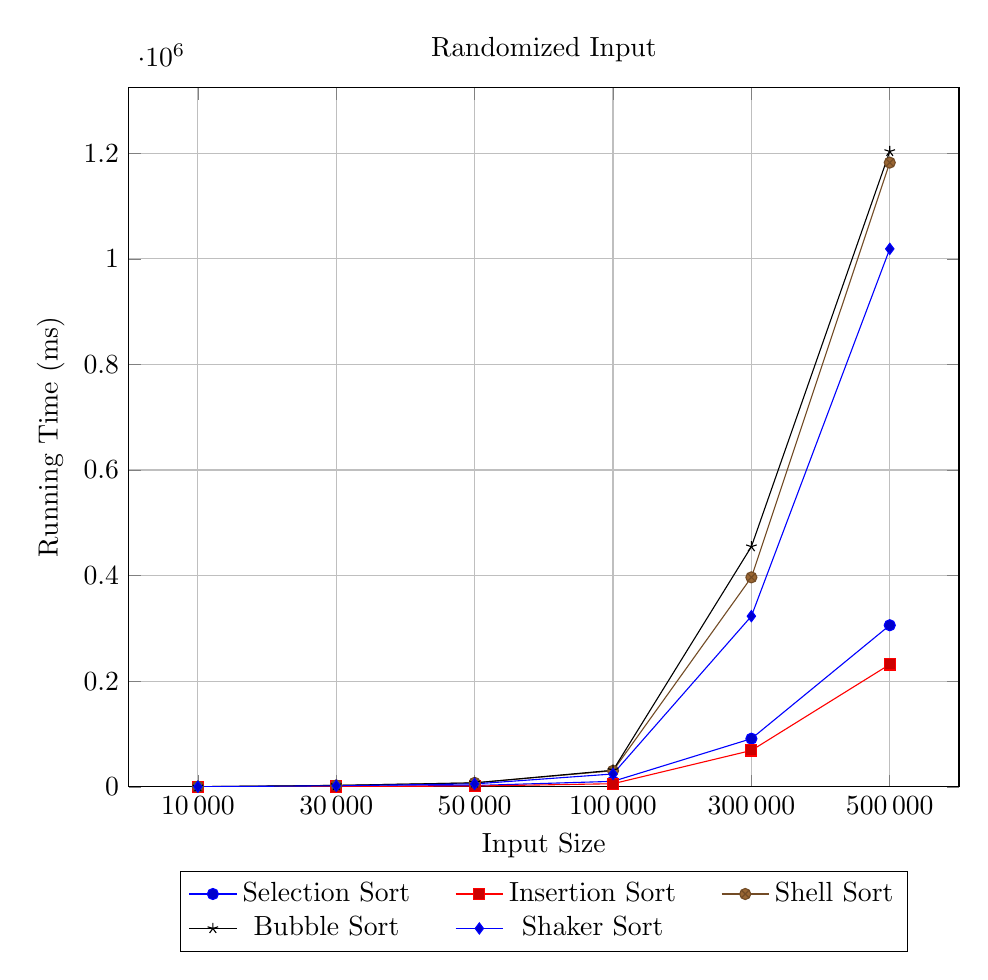
\begin{tikzpicture}
    \begin{axis}[
        width=\textwidth,
        title={Randomized Input},
        xlabel={Input Size},
        ylabel={Running Time (ms)},
        legend style={
            at={(0.5,-0.12)}, anchor=north, legend columns=3, 
            /tikz/every even column/.append style={column sep=0.5cm}
        },
        symbolic x coords={10\,000, 30\,000, 50\,000, 100\,000, 300\,000, 500\,000},
        xtick=data,
        ymin=0,
        grid=major,
    ]
    
    \addplot coordinates {(10\,000,110) (30\,000,870) (50\,000,2474) 
    (100\,000,10378) (300\,000,91156) (500\,000,306006)};
    \addlegendentry{Selection Sort}
    
    \addplot coordinates {(10\,000,58) (30\,000,504) (50\,000,1481) 
    (100\,000,5879) (300\,000,68865) (500\,000,231821)};
    \addlegendentry{Insertion Sort}
    
    \addplot coordinates {(10\,000,271) (30\,000,2692) (50\,000,7542) 
    (100\,000,30370) (300\,000,396729) (500\,000,1182221)};
    \addlegendentry{Shell Sort}
    
    \addplot coordinates {(10\,000,268) (30\,000,2639) (50\,000,7491) 
    (100\,000,31385) (300\,000,454882) (500\,000,1203413)};
    \addlegendentry{Bubble Sort}
    
    \addplot coordinates {(10\,000,219) (30\,000,1986) 
    (50\,000,5519) (100\,000,24340) (300\,000,323182) (500\,000,1018829)};
    \addlegendentry{Shaker Sort}
    
    \end{axis}
\end{tikzpicture}
\caption{Kết quả thực nghiệm với đầu vào có thứ tự ngẫu nhiên (Nhóm 1)}
\end{figure}

\begin{figure}[H]
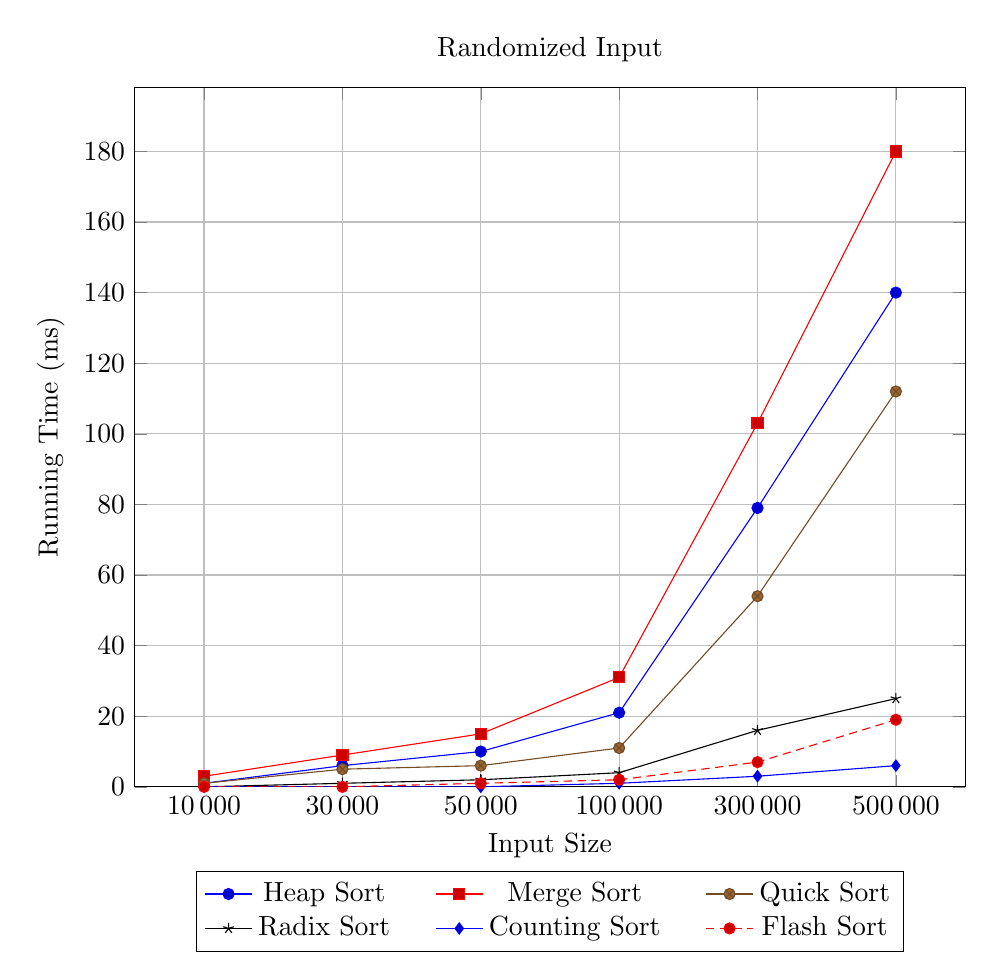
\begin{tikzpicture}
    \begin{axis}[
        width=\textwidth,
        title={Randomized Input},
        xlabel={Input Size},
        ylabel={Running Time (ms)},
        legend style={
            at={(0.5,-0.12)}, anchor=north, legend columns=3, 
            /tikz/every even column/.append style={column sep=0.5cm}
        },
        symbolic x coords={10\,000, 30\,000, 50\,000, 100\,000, 300\,000, 500\,000},
        xtick=data,
        ymin=0,
        grid=major,
    ]
    
    \addplot coordinates {(10\,000,1) (30\,000,6) (50\,000,10) 
    (100\,000,21) (300\,000,79) (500\,000,140)};
    \addlegendentry{Heap Sort}
    
    \addplot coordinates {(10\,000,3) (30\,000,9) (50\,000,15) 
    (100\,000,31) (300\,000,103) (500\,000,180)};
    \addlegendentry{Merge Sort}
    
    \addplot coordinates {(10\,000,1) (30\,000,5) (50\,000,6) 
    (100\,000,11) (300\,000,54) (500\,000,112)};
    \addlegendentry{Quick Sort}
    
    \addplot coordinates {(10\,000,0) (30\,000,1) (50\,000,2) 
    (100\,000,4) (300\,000,16) (500\,000,25)};
    \addlegendentry{Radix Sort}
    
    \addplot coordinates {(10\,000,0) (30\,000,0) (50\,000,0) 
    (100\,000,1) (300\,000,3) (500\,000,6)};
    \addlegendentry{Counting Sort}
    
    \addplot coordinates {(10\,000,0) (30\,000,0) (50\,000,1) 
    (100\,000,2) (300\,000,7) (500\,000,19)};
    \addlegendentry{Flash Sort}
    
    \end{axis}
\end{tikzpicture}
\caption{Kết quả thực nghiệm với đầu vào có thứ tự ngẫu nhiên (Nhóm 2)}
\end{figure}

\begin{itemize}[label=$\circ$]
    \item Thuật toán Bubble Sort có tốc độ chậm nhất với mọi kích thước 
    đầu vào, ngược lại Insertion Sort nhanh nhất trong nhóm thuật toán 
    có độ phức tạp trung bình là $O\left(n^2\right)$ cho dù số lượng phần tử có tăng 
    cao, thì thời gian thực thi vẫn không tăng quá nhiều. 
    \item Về nhóm thuật toán có độ phức tạp là $O\left(n\log{n}\right)$, 
    Merge Sort chậm đi rất nhiều khi kích thước đầu vào tăng lên do tiêu 
    tốn nhiều thời gian cho việc chia và trộn nhiều mảng con. Còn Quick 
    Sort mặc dù có tăng thời gian thực thi khi cỡ mẫu lớn hơn 100,000 
    nhưng vẫn nhanh nhất trong nhóm thuật toán này. 
\end{itemize}

\pagebreak

\begin{itemize}[label=$\circ$]
    \item Với các thuật toán còn lại, Counting Sort giữ vị trí thứ nhất 
    nhưng bị hạn chế về kiểu dữ liệu, như với số thực hoặc số nguyên lớn 
    cần phải xử lý một cách khéo léo. Mặc khác, Flash Sort có thể xử lý 
    đa dạng kiểu dữ liệu và tốc độ cũng đáng kể nhưng phụ thuộc vào sự 
    phân phối của dữ liệu đầu vào và quá trình cài đặt khá phức tạp.
\end{itemize}

$\bullet$ \textbf{Với đầu vào có thứ tự gần được sắp xếp}

\begin{figure}[H]
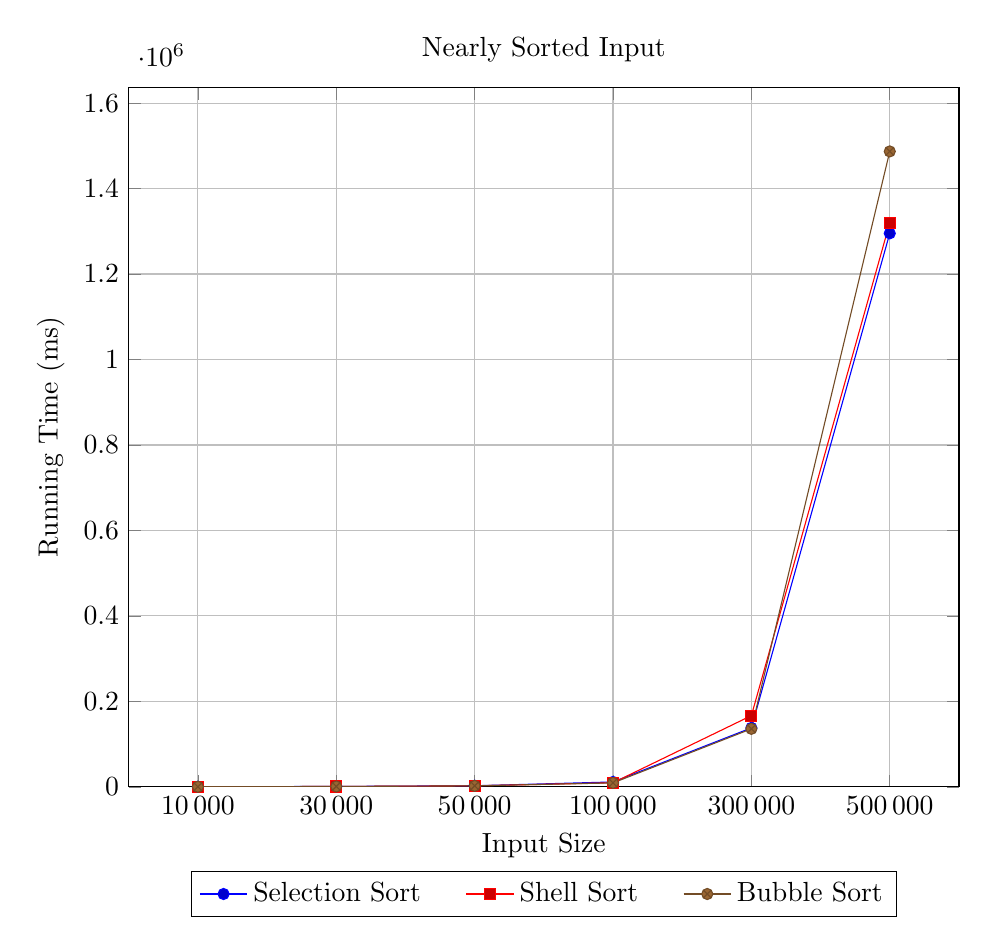
\begin{tikzpicture}
    \begin{axis}[
        width=\textwidth,
        title={Nearly Sorted Input},
        xlabel={Input Size},
        ylabel={Running Time (ms)},
        legend style={
            at={(0.5,-0.12)}, anchor=north, legend columns=3, 
            /tikz/every even column/.append style={column sep=0.5cm}
        },
        symbolic x coords={10\,000, 30\,000, 50\,000, 100\,000, 300\,000, 500\,000},
        xtick=data,
        ymin=0,
        grid=major,
    ]
    
    \addplot coordinates {(10\,000,106) (30\,000,868) (50\,000,2472) 
    (100\,000,11396) (300\,000,137957) (500\,000,1295243)};
    \addlegendentry{Selection Sort}
    
    \addplot coordinates {(10\,000,96) (30\,000,812) (50\,000,2290) 
    (100\,000,9538) (300\,000,166585) (500\,000,1319995)};
    \addlegendentry{Shell Sort}
    
    \addplot coordinates {(10\,000,94) (30\,000,828) (50\,000,2259) 
    (100\,000,9164) (300\,000,135698) (500\,000,1486996)};
    \addlegendentry{Bubble Sort}
    
    \end{axis}
\end{tikzpicture}
\caption{Kết quả thực nghiệm với đầu vào có thứ tự gần được sắp xếp (Nhóm 1)}
\end{figure}

\begin{figure}[H]
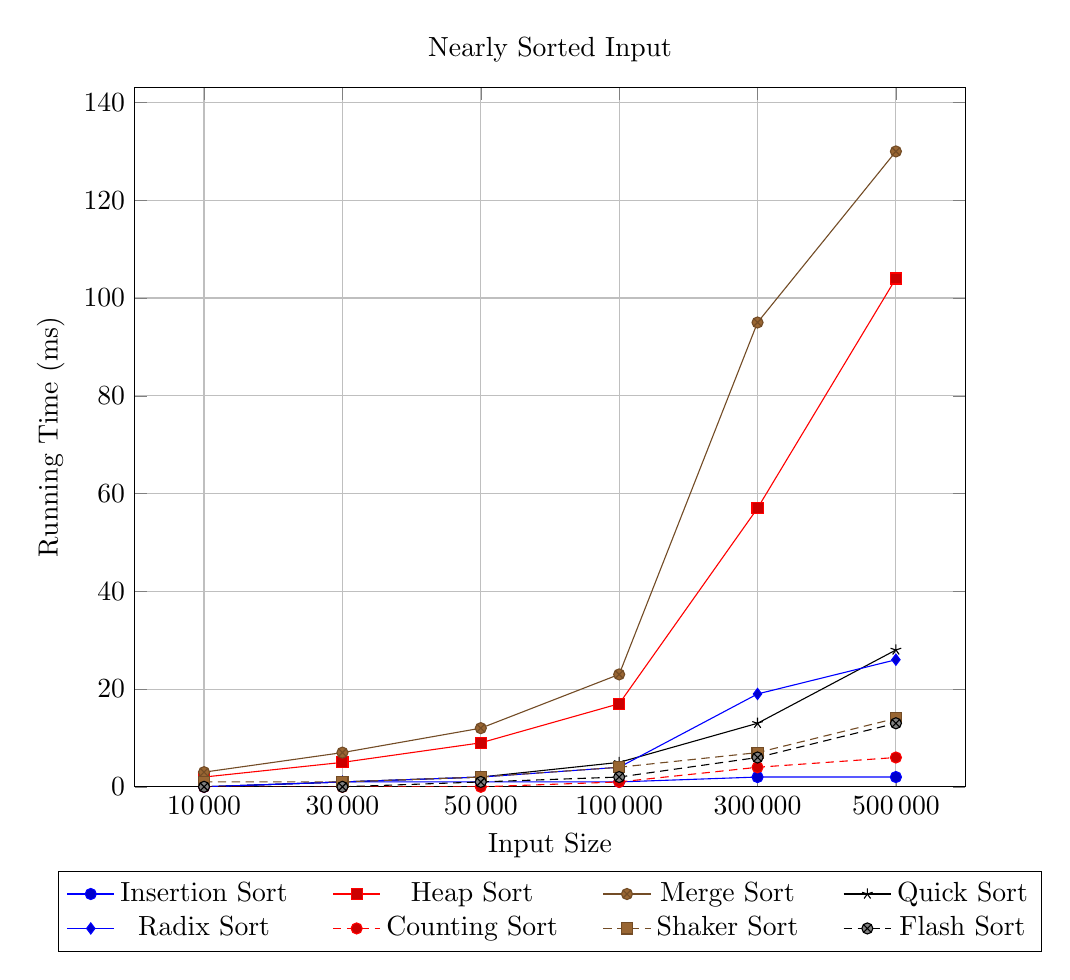
\begin{tikzpicture}
    \begin{axis}[
        width=\textwidth,
        title={Nearly Sorted Input},
        xlabel={Input Size},
        ylabel={Running Time (ms)},
        legend style={
            at={(0.5,-0.12)}, anchor=north, legend columns=4, 
            /tikz/every even column/.append style={column sep=0.5cm}
        },
        symbolic x coords={10\,000, 30\,000, 50\,000, 100\,000, 300\,000, 500\,000},
        xtick=data,
        ymin=0,
        grid=major,
    ]
    
    \addplot coordinates {(10\,000,0) (30\,000,1) (50\,000,1) 
    (100\,000,1) (300\,000,2) (500\,000,2)};
    \addlegendentry{Insertion Sort}
    
    \addplot coordinates {(10\,000,2) (30\,000,5) (50\,000,9) 
    (100\,000,17) (300\,000,57) (500\,000,104)};
    \addlegendentry{Heap Sort}
    
    \addplot coordinates {(10\,000,3) (30\,000,7) (50\,000,12) 
    (100\,000,23) (300\,000,95) (500\,000,130)};
    \addlegendentry{Merge Sort}
    
    \addplot coordinates {(10\,000,0) (30\,000,1) (50\,000,2) 
    (100\,000,5) (300\,000,13) (500\,000,28)};
    \addlegendentry{Quick Sort}
    
    \addplot coordinates {(10\,000,0) (30\,000,1) (50\,000,2) 
    (100\,000,4) (300\,000,19) (500\,000,26)};
    \addlegendentry{Radix Sort}
    
    \addplot coordinates {(10\,000,0) (30\,000,0) (50\,000,0) 
    (100\,000,1) (300\,000,4) (500\,000,6)};
    \addlegendentry{Counting Sort}
    
    \addplot coordinates {(10\,000,1) (30\,000,1) (50\,000,2) 
    (100\,000,4) (300\,000,7) (500\,000,14)};
    \addlegendentry{Shaker Sort}
    
    \addplot coordinates {(10\,000,0) (30\,000,0) (50\,000,1) 
    (100\,000,2) (300\,000,6) (500\,000,13)};
    \addlegendentry{Flash Sort}
    
    \end{axis}
\end{tikzpicture}
\caption{Kết quả thực nghiệm với đầu vào có thứ tự gần được sắp xếp (Nhóm 2)}
\end{figure}

\begin{itemize}[label=$\circ$]
    \item Các thuật toán như Selection Sort, Shell Sort, Bubble Sort, 
    Merge Sort và Heap Sort đều không có nhiều cải thiện. Ngược lại, 
    Shaker Sort, Insertion Sort và Quick Sort đã giảm đáng kể thời gian 
    thực thi xuống ngang bằng với nhóm thuật toán còn lại, thậm chí 
    Insertion Sort còn giữ vị trí nhanh nhất do chỉ cần đưa một vài 
    phần tử nằm sai vị trí về đúng chỗ.
\end{itemize}

\pagebreak

$\bullet$ \textbf{Với đầu vào có thứ tự đã được sắp xếp}

\begin{figure}[H]
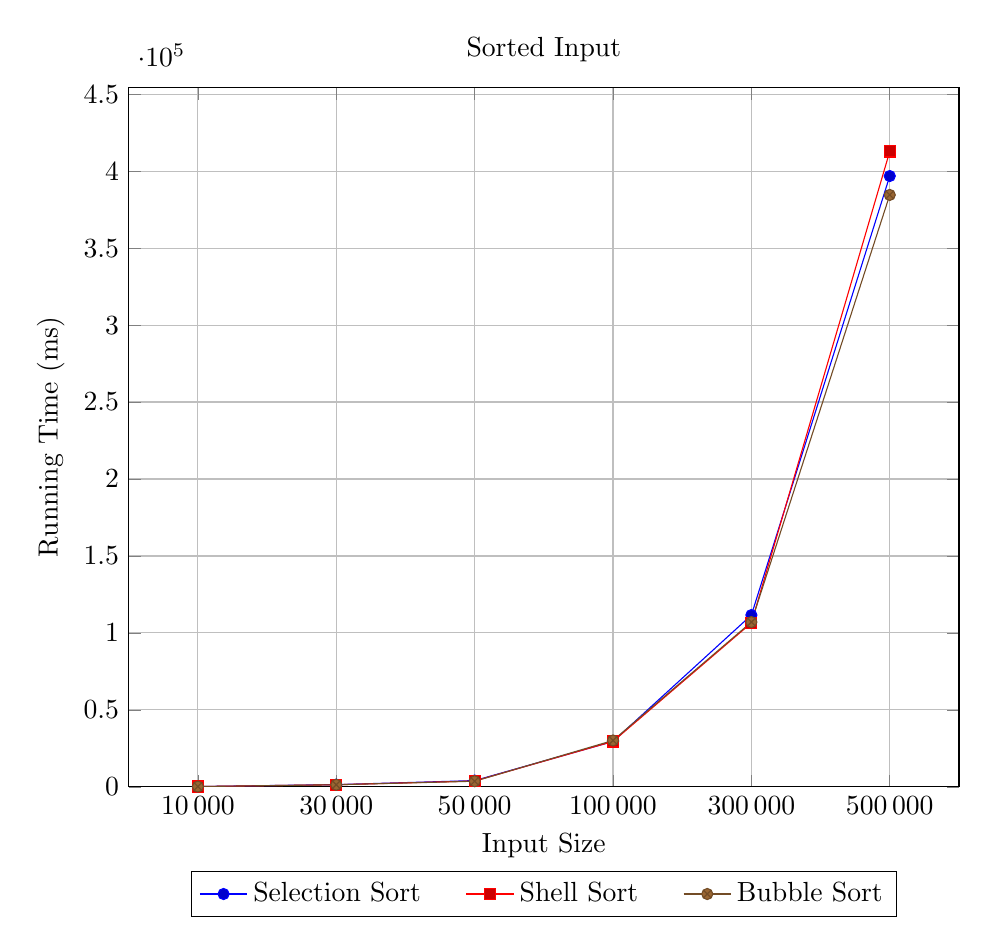
\begin{tikzpicture}
    \begin{axis}[
        width=\textwidth,
        title={Sorted Input},
        xlabel={Input Size},
        ylabel={Running Time (ms)},
        legend style={
            at={(0.5,-0.12)}, anchor=north, legend columns=3, 
            /tikz/every even column/.append style={column sep=0.5cm}
        },
        symbolic x coords={10\,000, 30\,000, 50\,000, 100\,000, 300\,000, 500\,000},
        xtick=data,
        ymin=0,
        grid=major,
    ]

    \addplot coordinates {(10\,000,182) (30\,000,1426) (50\,000,4059) 
    (100\,000,29478) (300\,000,111585) (500\,000,396841)};
    \addlegendentry{Selection Sort}
    
    \addplot coordinates {(10\,000,179) (30\,000,1349) (50\,000,3786) 
    (100\,000,29503) (300\,000,106498) (500\,000,412844)};
    \addlegendentry{Shell Sort}
    
    \addplot coordinates {(10\,000,180) (30\,000,1346) (50\,000,3636) 
    (100\,000,30120) (300\,000,107040) (500\,000,384574)};
    \addlegendentry{Bubble Sort}
    \end{axis}
\end{tikzpicture}
\caption{Kết quả thực nghiệm với đầu vào có thứ tự đã được sắp xếp (Nhóm 1)}
\end{figure}

\begin{figure}[H]
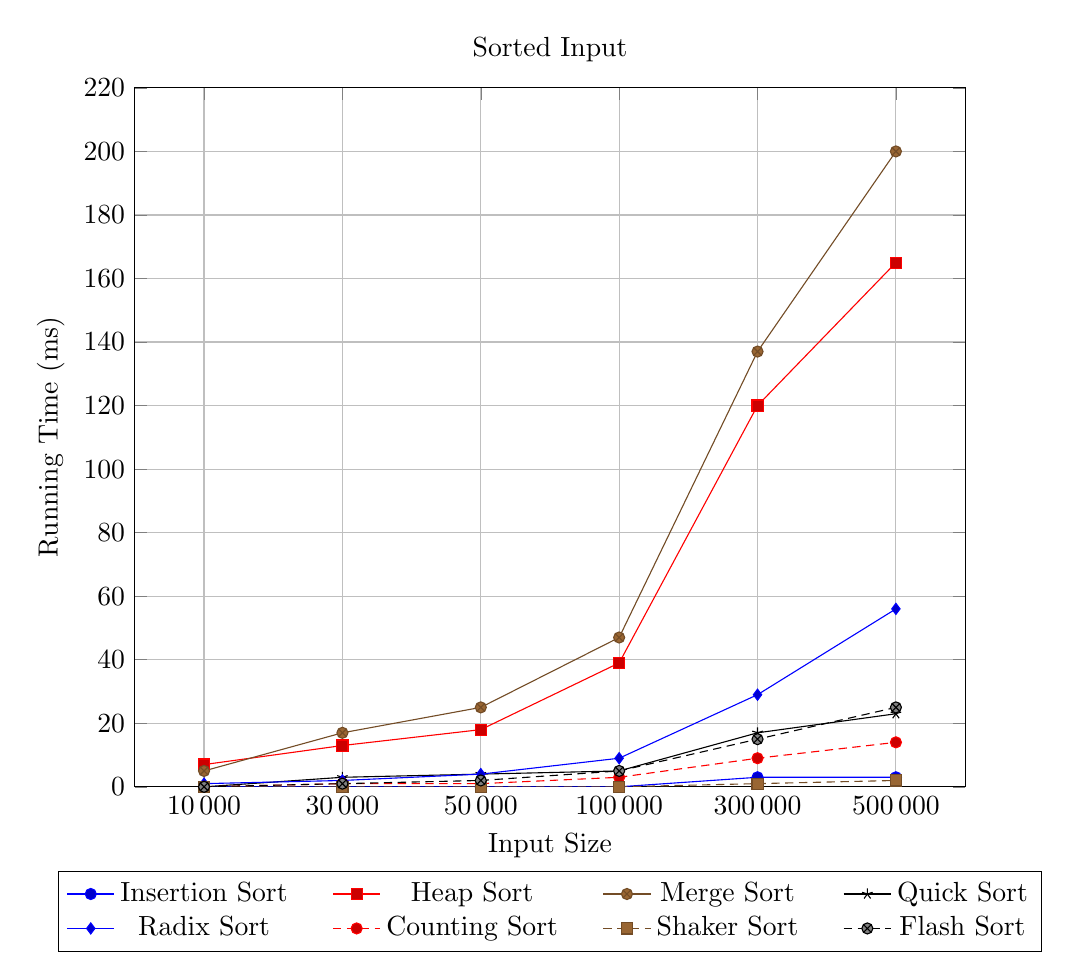
\begin{tikzpicture}
    \begin{axis}[
        width=\textwidth,
        title={Sorted Input},
        xlabel={Input Size},
        ylabel={Running Time (ms)},
        legend style={
            at={(0.5,-0.12)}, anchor=north, legend columns=4, 
            /tikz/every even column/.append style={column sep=0.5cm}
        },
        symbolic x coords={10\,000, 30\,000, 50\,000, 100\,000, 300\,000, 500\,000},
        xtick=data,
        ymin=0,
        grid=major,
    ]
    
    \addplot coordinates {(10\,000,0) (30\,000,0) (50\,000,0) 
    (100\,000,0) (300\,000,3) (500\,000,3)};
    \addlegendentry{Insertion Sort}
    
    \addplot coordinates {(10\,000,7) (30\,000,13) (50\,000,18) 
    (100\,000,39) (300\,000,120) (500\,000,165)};
    \addlegendentry{Heap Sort}
    
    \addplot coordinates {(10\,000,5) (30\,000,17) (50\,000,25) 
    (100\,000,47) (300\,000,137) (500\,000,200)};
    \addlegendentry{Merge Sort}
    
    \addplot coordinates {(10\,000,0) (30\,000,3) (50\,000,4) 
    (100\,000,5) (300\,000,17) (500\,000,23)};
    \addlegendentry{Quick Sort}
    
    \addplot coordinates {(10\,000,1) (30\,000,2) (50\,000,4) 
    (100\,000,9) (300\,000,29) (500\,000,56)};
    \addlegendentry{Radix Sort}
    
    \addplot coordinates {(10\,000,0) (30\,000,1) (50\,000,1) 
    (100\,000,3) (300\,000,9) (500\,000,14)};
    \addlegendentry{Counting Sort}
    
    \addplot coordinates {(10\,000,0) (30\,000,0) (50\,000,0) 
    (100\,000,0) (300\,000,1) (500\,000,2)};
    \addlegendentry{Shaker Sort}
    
    \addplot coordinates {(10\,000,0) (30\,000,1) (50\,000,2) 
    (100\,000,5) (300\,000,15) (500\,000,25)};
    \addlegendentry{Flash Sort}
    
    \end{axis}
\end{tikzpicture}
\caption{Kết quả thực nghiệm với đầu vào có thứ tự đã được sắp xếp (Nhóm 2)}
\end{figure}

\begin{itemize}[label=$\circ$]
    \item Trong nhóm thuật toán có độ phức tạp $O\left(n^2\right)$ thì 
    Insertion Sort và Shaker Sort có tốc độ rất nhanh và hầu như là không 
    tốn thời gian với 100,000 phần tử. Ngược lại, 2 thuật toán còn lại 
    là Select Sort và Bubble Sort thì lại tốn khá nhiều thời gian và có 
    thời gian chạy không chênh lệch nhiều so với nhau.
    \item Trong nhóm thuật toán có độ phức tạp $O\left(n\log{n}\right)$ 
    thì Shell Sort lại dường như tốn rất nhiều thời gian tương đương với 
    một số thuật toán có độ phức tạp trung bình là $O\left(n^2\right)$, 
    còn Quick Sort là thuật toán có thời gian chạy nhanh nhất, Heap Sort 
    thì nhanh hơn Merge Sort một chút.
    \item Trong nhóm thuật toán còn lại thì Counting Sort vẫn có thời 
    gian chạy nhanh nhất, còn Radix Sort thì có thời gian chạy chậm nhất.
\end{itemize}

$\bullet$ \textbf{Với đầu vào có thứ tự được sắp xếp ngược}

\begin{figure}[H]
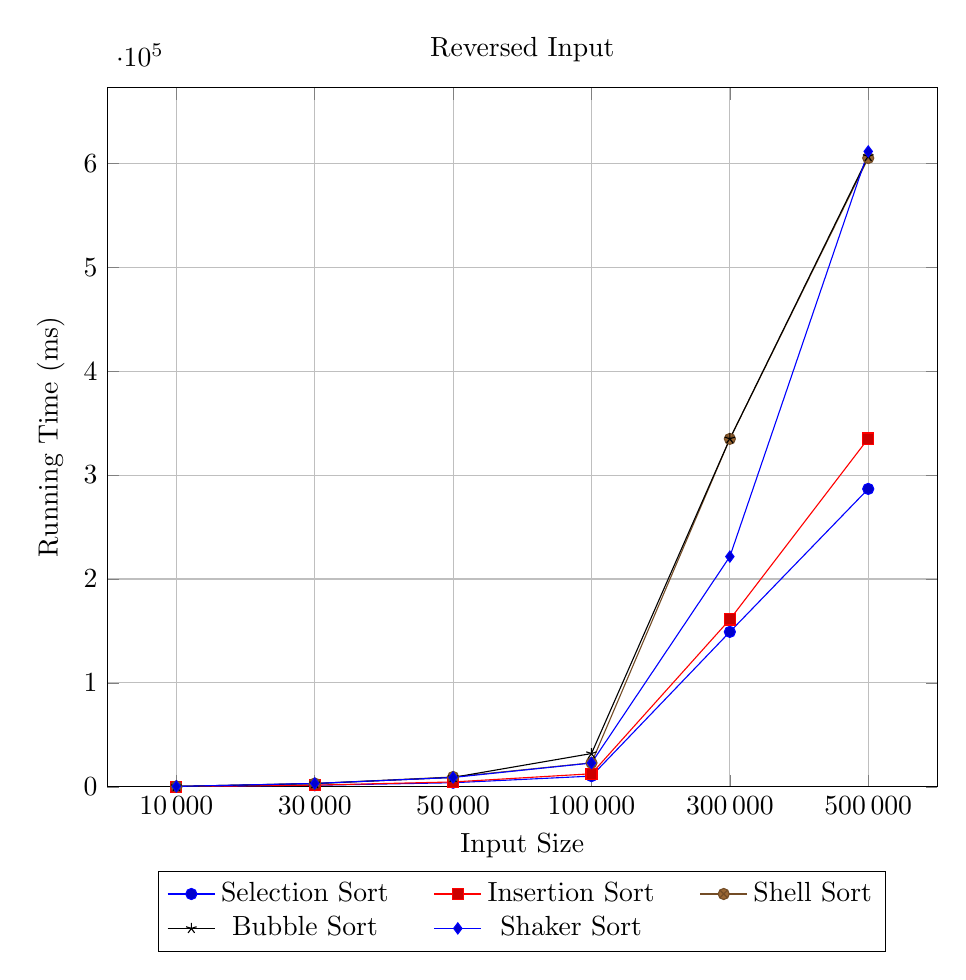
\begin{tikzpicture}
    \begin{axis}[
        width=\textwidth,
        title={Reversed Input},
        xlabel={Input Size},
        ylabel={Running Time (ms)},
        legend style={
            at={(0.5,-0.12)}, anchor=north, legend columns=3, 
            /tikz/every even column/.append style={column sep=0.5cm}
        },
        symbolic x coords={10\,000, 30\,000, 50\,000, 100\,000, 300\,000, 500\,000},
        xtick=data,
        ymin=0,
        grid=major,
    ]
    
    \addplot coordinates {(10\,000,175) (30\,000,1477) (50\,000,3924) 
    (100\,000,10289) (300\,000,149091) (500\,000,286666)};
    \addlegendentry{Selection Sort}
    
    \addplot coordinates {(10\,000,202) (30\,000,1630) (50\,000,4686) 
    (100\,000,12560) (300\,000,161038) (500\,000,335113)};
    \addlegendentry{Insertion Sort}
    
    \addplot coordinates {(10\,000,383) (30\,000,3158) (50\,000,9485) 
    (100\,000,23060) (300\,000,334815) (500\,000,605040)};
    \addlegendentry{Shell Sort}
    
    \addplot coordinates {(10\,000,373) (30\,000,3116) (50\,000,9043) 
    (100\,000,32013) (300\,000,334914) (500\,000,606656)};
    \addlegendentry{Bubble Sort}
    
    \addplot coordinates {(10\,000,385) (30\,000,3255) (50\,000,9005) 
    (100\,000,22892) (300\,000,221549) (500\,000,611441)};
    \addlegendentry{Shaker Sort}
    
    \end{axis}
\end{tikzpicture}
\caption{Kết quả thực nghiệm với đầu vào có thứ tự được sắp xếp ngược (Nhóm 1)}
\end{figure}

\begin{figure}[H]
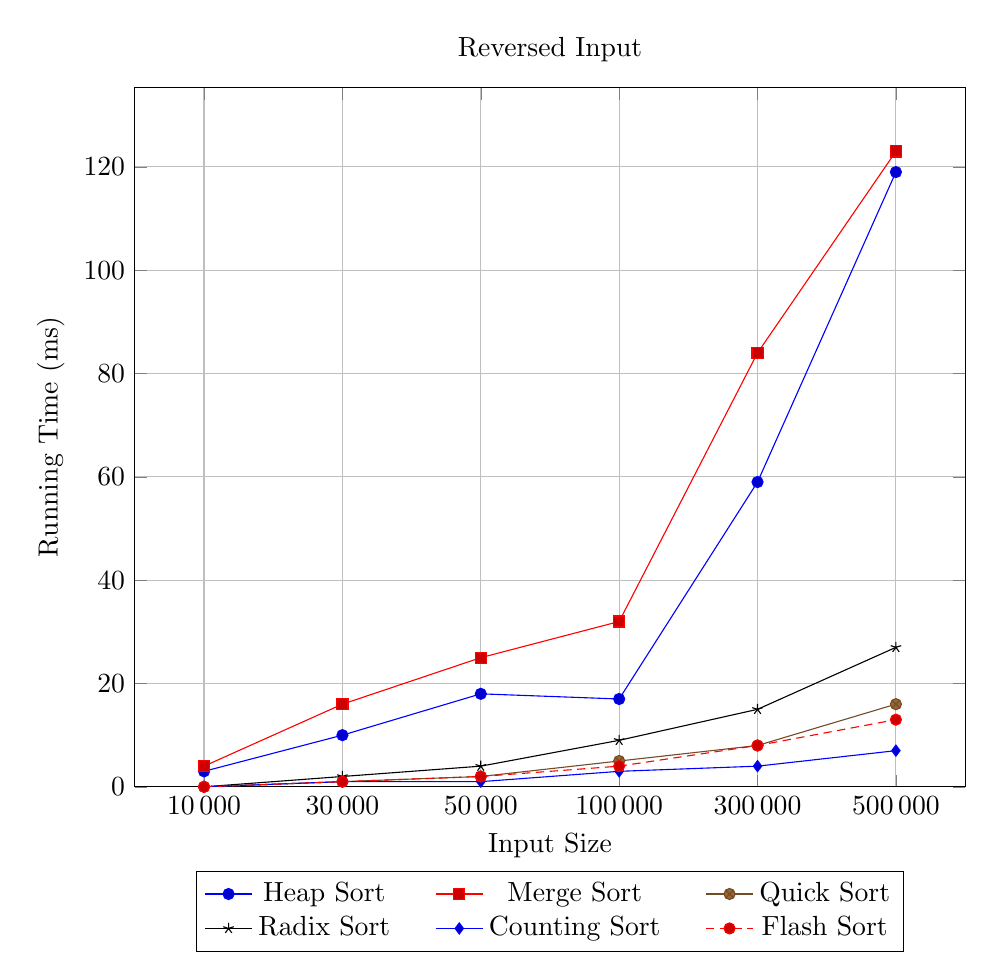
\begin{tikzpicture}
    \begin{axis}[
        width=\textwidth,
        title={Reversed Input},
        xlabel={Input Size},
        ylabel={Running Time (ms)},
        legend style={
            at={(0.5,-0.12)}, anchor=north, legend columns=3, 
            /tikz/every even column/.append style={column sep=0.5cm}
        },
        symbolic x coords={10\,000, 30\,000, 50\,000, 100\,000, 300\,000, 500\,000},
        xtick=data,
        ymin=0,
        grid=major,
    ]
    
    \addplot coordinates {(10\,000,3) (30\,000,10) (50\,000,18) 
    (100\,000,17) (300\,000,59) (500\,000,119)};
    \addlegendentry{Heap Sort}
    
    \addplot coordinates {(10\,000,4) (30\,000,16) (50\,000,25) 
    (100\,000,32) (300\,000,84) (500\,000,123)};
    \addlegendentry{Merge Sort}
    
    \addplot coordinates {(10\,000,0) (30\,000,1) (50\,000,2) 
    (100\,000,5) (300\,000,8) (500\,000,16)};
    \addlegendentry{Quick Sort}
    
    \addplot coordinates {(10\,000,0) (30\,000,2) (50\,000,4) 
    (100\,000,9) (300\,000,15) (500\,000,27)};
    \addlegendentry{Radix Sort}
    
    \addplot coordinates {(10\,000,0) (30\,000,1) (50\,000,1) 
    (100\,000,3) (300\,000,4) (500\,000,7)};
    \addlegendentry{Counting Sort}
    
    \addplot coordinates {(10\,000,0) (30\,000,1) (50\,000,2) 
    (100\,000,4) (300\,000,8) (500\,000,13)};
    \addlegendentry{Flash Sort}
    
    \end{axis}
\end{tikzpicture}
\caption{Kết quả thực nghiệm với đầu vào có thứ tự được sắp xếp ngược (Nhóm 2)}
\end{figure}

\begin{itemize}[label=$\circ$]
    \item Các thuật toán như Selection Sort, Shell Sort, Bubble Sort, 
    Merge Sort, và Heap Sort đều thể hiện thời gian thực thi cao, đặc 
    biệt là nhóm các thuật toán có độ phức tạp thời gian trung bình là 
    $O\left(n^2\right)$. Những thuật toán như Bubble Sort và Shaker Sort 
    trở nên chậm đáng kể do cần nhiều phép hoán đổi, trong khi Selection 
    Sort duy trì hiệu suất ổn định nhưng vẫn kém hiệu quả vì phải duyệt 
    toàn bộ danh sách để tìm giá trị nhỏ nhất.
    \item Ngược lại, nhóm thuật toán có độ phức tạp trung bình là 
    $O\left(n\log{n}\right)$ như Quick Sort, Merge Sort và Heap Sort thể 
    hiện hiệu suất vượt trội hơn, với Merge Sort và Heap Sort ổn định hơn 
    so với Quick Sort do đặc thù phân chia dữ liệu của chúng.
    \item Đặc biệt, các thuật toán còn lại như Counting Sort và Flash 
    Sort cho thấy thời gian thực thi thấp nhất trong các biểu đồ, chứng 
    minh tính vượt trội khi xử lý các dữ liệu lớn ngay cả trong trường 
    hợp xấu nhất.
\end{itemize}

\subsubsection{Về số phép so sánh}

$\bullet$ \textbf{Với đầu vào có thứ tự ngẫu nhiên}

\begin{figure}[H]
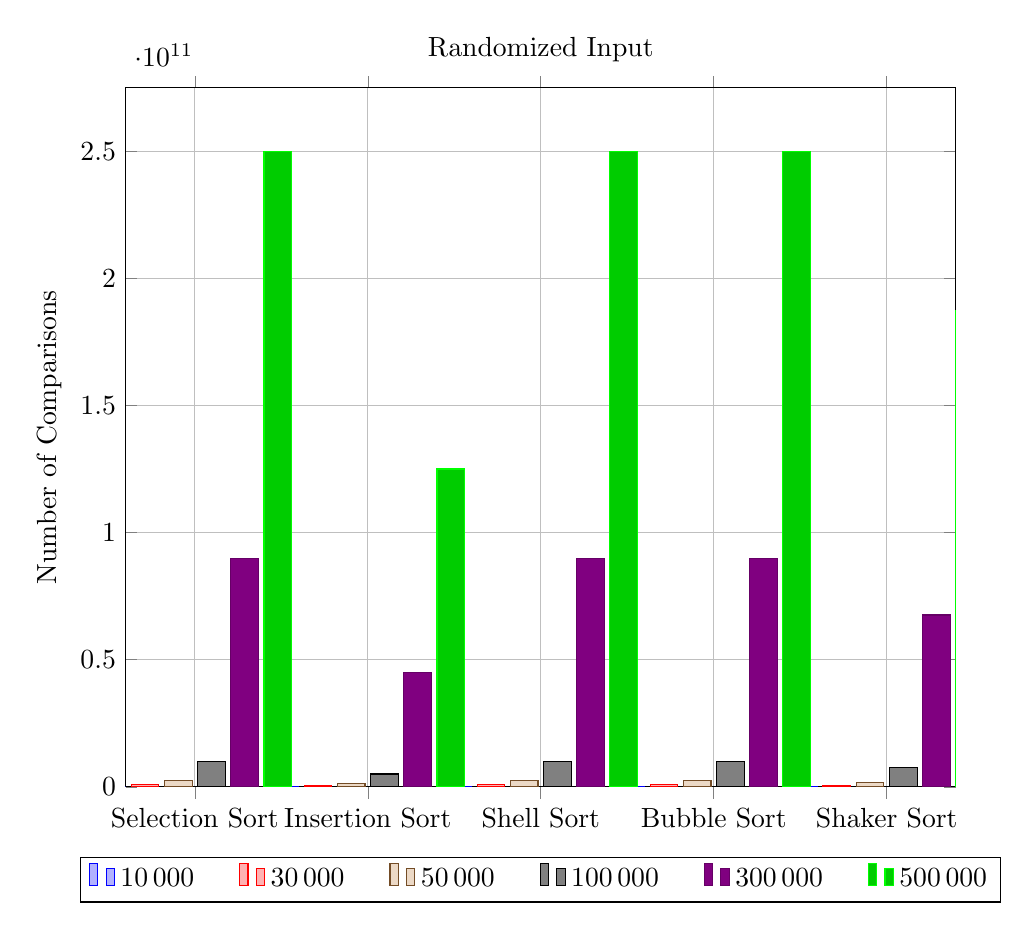
\begin{tikzpicture}
    \begin{axis}[
        width=\textwidth,
        title={Randomized Input},
        ybar,
        ymin=0,
        grid=major,
        legend style={
            at={(0.5,-0.1)}, anchor=north, legend columns=-1,
            /tikz/every even column/.append style={column sep=0.5cm}
        },
        ylabel={Number of Comparisons},
        symbolic x coords={
            Selection Sort, Insertion Sort, Shell Sort, Bubble Sort, 
            Shaker Sort
        },
        xtick=data,
    ]
    \addplot coordinates {(Selection Sort,100009999) 
        (Insertion Sort,49852722) (Shell Sort,100009999) 
        (Bubble Sort,100009999) (Shaker Sort,75877345)};
    \addplot coordinates {(Selection Sort,900029999) 
        (Insertion Sort,450424387) (Shell Sort,900029999) 
        (Bubble Sort,900029999) (Shaker Sort,678034901)};
    \addplot coordinates {(Selection Sort,2500049999) 
        (Insertion Sort,1244875082) (Shell Sort,2500049999) 
        (Bubble Sort,2500049999) (Shaker Sort,1868558231)};
    \addplot coordinates {(Selection Sort,10000099999) 
        (Insertion Sort,5026592949) (Shell Sort,10000099999) 
        (Bubble Sort,10000099999) (Shaker Sort,7519014091)};
    \addplot coordinates {(Selection Sort,90000299999) 
        (Insertion Sort,44937080911) (Shell Sort,90000299999) 
        (Bubble Sort,90000299999) (Shaker Sort,67598742089)};
    \addplot coordinates {(Selection Sort,250000499999) 
        (Insertion Sort,125044404674) (Shell Sort,250000499999) 
        (Bubble Sort,250000499999) (Shaker Sort,187569730819)};
        \legend{10\,000, 30\,000, 50\,000, 100\,000, 300\,000, 500\,000}
    \end{axis}
\end{tikzpicture}
\caption{Kết quả thực nghiệm với đầu vào có thứ tự ngẫu nhiên (Nhóm 1)}
\end{figure}

\begin{figure}[H]
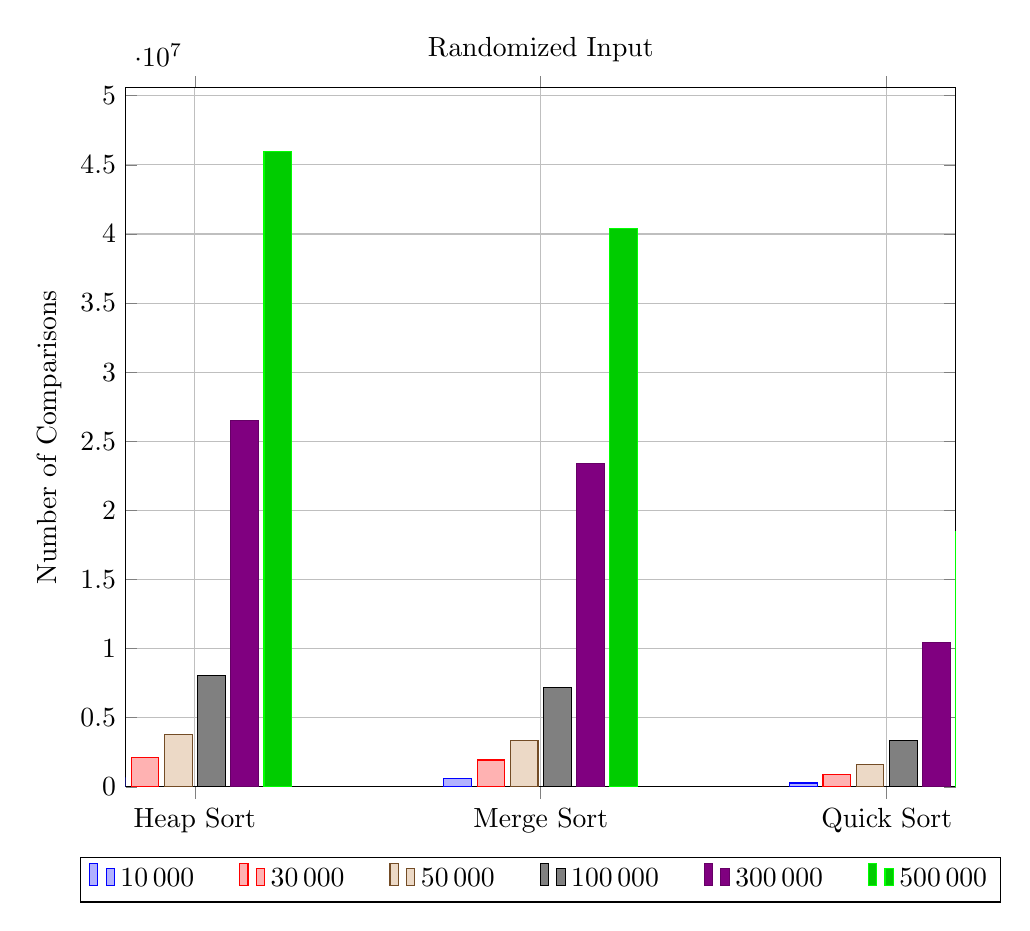
\begin{tikzpicture}
    \begin{axis}[
        width=\textwidth,
        title={Randomized Input},
        ybar,
        ymin=0,
        grid=major,
        legend style={
            at={(0.5,-0.1)}, anchor=north, legend columns=-1,
            /tikz/every even column/.append style={column sep=0.5cm}
        },
        ylabel={Number of Comparisons},
        symbolic x coords={Heap Sort, Merge Sort, Quick Sort},
        xtick=data,
    ]
    \addplot coordinates {(Heap Sort,638425) 
        (Merge Sort,583832) (Quick Sort,276045)};
    \addplot coordinates {(Heap Sort,2150786) 
        (Merge Sort,1937240) (Quick Sort,916849)};
    \addplot coordinates {(Heap Sort,3771772) 
        (Merge Sort,3383319) (Quick Sort,1636700)};
    \addplot coordinates {(Heap Sort,8044992) 
        (Merge Sort,7166010) (Quick Sort,3341712)};
    \addplot coordinates {(Heap Sort,26487787) 
        (Merge Sort,23383601) (Quick Sort,10434674)};
    \addplot coordinates {(Heap Sort,45972193) 
        (Merge Sort,40383061) (Quick Sort,18476753)};
    \legend{10\,000, 30\,000, 50\,000, 100\,000, 300\,000, 500\,000}
    \end{axis}
\end{tikzpicture}
\caption{Kết quả thực nghiệm với đầu vào có thứ tự ngẫu nhiên (Nhóm 2)}
\end{figure}

\begin{figure}[H]
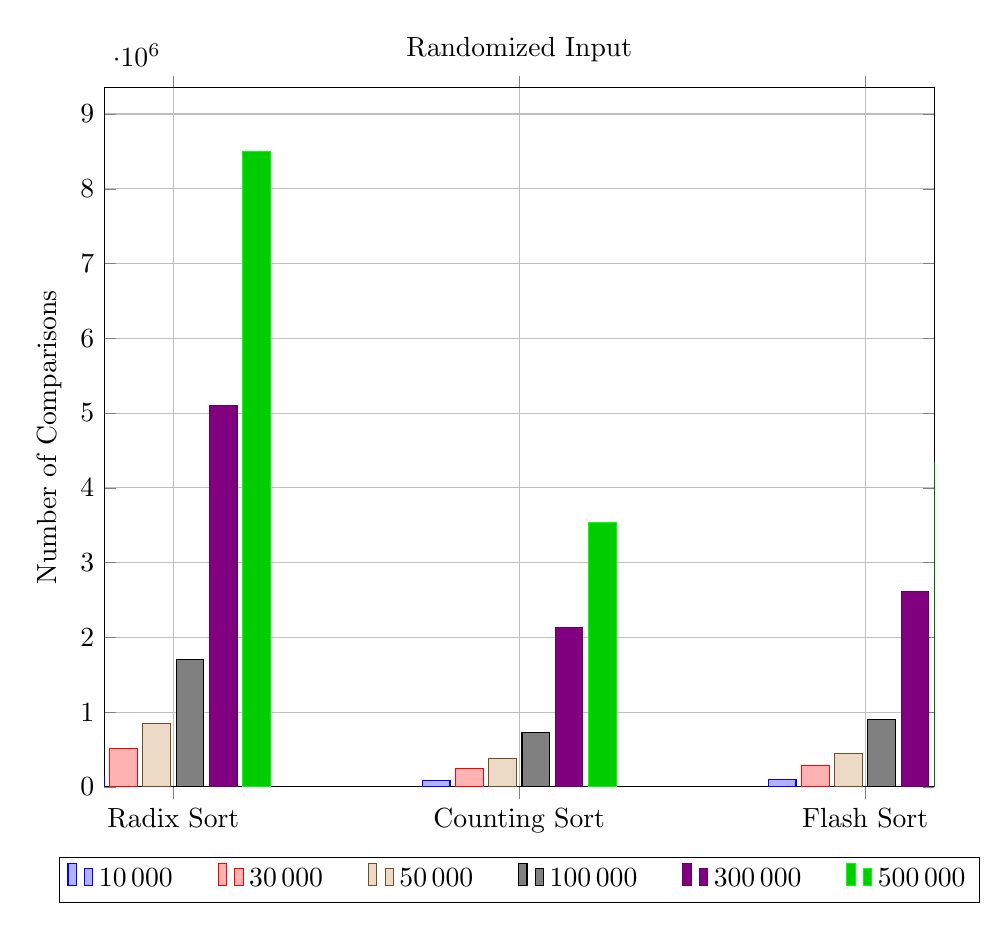
\begin{tikzpicture}
    \begin{axis}[
        width=\textwidth,
        title={Randomized Input},
        ybar,
        ymin=0,
        grid=major,
        legend style={
            at={(0.5,-0.1)}, anchor=north, legend columns=-1,
            /tikz/every even column/.append style={column sep=0.5cm}
        },
        ylabel={Number of Comparisons},
        symbolic x coords={Radix Sort, Counting Sort, Flash Sort},
        xtick=data,
    ]
    \addplot coordinates {(Radix Sort,140056) 
        (Counting Sort,80000) (Flash Sort,97658)};
    \addplot coordinates {(Radix Sort,510070) 
        (Counting Sort,240000) (Flash Sort,285201)};
    \addplot coordinates {(Radix Sort,850070) 
        (Counting Sort,382769) (Flash Sort,451390)};
    \addplot coordinates {(Radix Sort,1700070) 
        (Counting Sort,732769) (Flash Sort,905677)};
    \addplot coordinates {(Radix Sort,5100070) 
        (Counting Sort,2132769) (Flash Sort,2611012)};
    \addplot coordinates {(Radix Sort,8500070) 
        (Counting Sort,3532769) (Flash Sort,4335083)};
    \legend{10\,000, 30\,000, 50\,000, 100\,000, 300\,000, 500\,000}
    \end{axis}
\end{tikzpicture}
\caption{Kết quả thực nghiệm với đầu vào có thứ tự ngẫu nhiên (Nhóm 3)}
\end{figure}

\begin{itemize}[label=$\circ$]
    \item Có thể nhận xét rằng số phép so sánh giữa các thuật toán sắp 
    xếp thay đổi đáng kể tùy thuộc vào độ phức tạp về thời gian của từng 
    thuật toán. Nhóm các thuật toán có số phép so sánh lớn nhất bao gồm 
    Selection Sort, Insertion Sort, Shell Sort, Bubble Sort và Shaker 
    Sort do có độ phức tạp trung bình là $O\left(n^2\right)$. Trong đó, 
    cả 3 thuật toán gồm Selection Sort, Shell Sort, Bubble Sort đều có 
    số phép so sánh bằng nhau và lớn nhất so với 8 thuật toán còn lại. 
    Điều này dẫn đến số phép so sánh tăng nhanh khi kích thước mảng lớn, 
    đặc biệt là ở các mảng kích thước 300000 và 500000, với cột biểu đồ 
    vượt trội hơn hẳn so với các thuật toán khác.
\end{itemize}

\pagebreak

\begin{itemize}[label=$\circ$]
	\item Trong khi đó, nhóm thuật toán có hiệu suất trung bình như Heap 
    Sort, Merge Sort, và Quick Sort hoạt động hiệu quả hơn nhờ độ phức 
    tạp có độ phức tạp trung bình là $O\left(n\log{n}\right)$. Quick Sort 
    có số phép so sánh thấp hơn so với Heap Sort và Merge Sort, cho thấy 
    ưu thế rõ rệt khi xử lý trên mảng ngẫu nhiên.
	\item Cuối cùng, nhóm thuật toán có số phép so sánh thấp nhất bao 
    gồm Radix Sort, Counting Sort, và Flash Sort, nhờ đặc điểm không dựa 
    trên các phép so sánh với độ phức tạp lần lượt là $O\left(d\times\left(n+k\right)\right)$, 
    $O\left(n+k\right)$ và $O\left(n\right)$. Counting Sort đặc biệt nổi bật với 
    số phép so sánh thấp nhất trong nhóm này và thấp nhất trong 11 thuật 
    toán.
\end{itemize}

$\bullet$ \textbf{Với đầu vào có thứ tự gần được sắp xếp}

\begin{figure}[H]
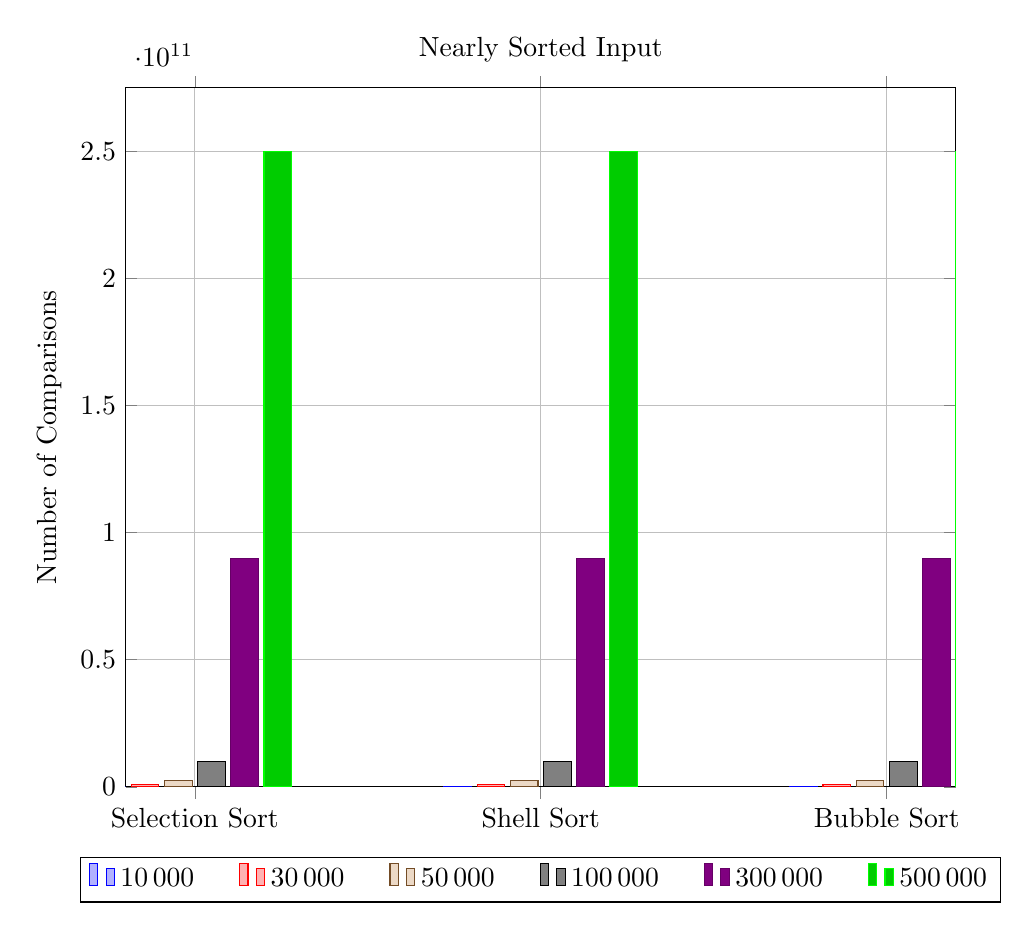
\begin{tikzpicture}
    \begin{axis}[
        width=\textwidth,
        title={Nearly Sorted Input},
        ybar,
        ymin=0,
        grid=major,
        legend style={
            at={(0.5,-0.1)}, anchor=north, legend columns=-1,
            /tikz/every even column/.append style={column sep=0.5cm}
        },
        ylabel={Number of Comparisons},
        symbolic x coords={Selection Sort, Shell Sort, Bubble Sort},
        xtick=data,
    ]
    \addplot coordinates {(Selection Sort,100009999) 
        (Shell Sort,100009999) (Bubble Sort,100009999)};
    \addplot coordinates {(Selection Sort,900029999) 
        (Shell Sort,900029999) (Bubble Sort,900029999)};
    \addplot coordinates {(Selection Sort,2500049999) 
        (Shell Sort,2500049999) (Bubble Sort,2500049999)};
    \addplot coordinates {(Selection Sort,10000099999) 
        (Shell Sort,10000099999) (Bubble Sort,10000099999)};
    \addplot coordinates {(Selection Sort,90000299999) 
        (Shell Sort,90000299999) (Bubble Sort,90000299999)};
    \addplot coordinates {(Selection Sort,250000499999) 
        (Shell Sort,250000499999) (Bubble Sort,250000499999)};
    \legend{10\,000, 30\,000, 50\,000, 100\,000, 300\,000, 500\,000}
    \end{axis}
\end{tikzpicture}
\caption{Kết quả thực nghiệm với đầu vào có thứ tự gần được sắp xếp (Nhóm 1)}
\end{figure}

\begin{figure}[H]
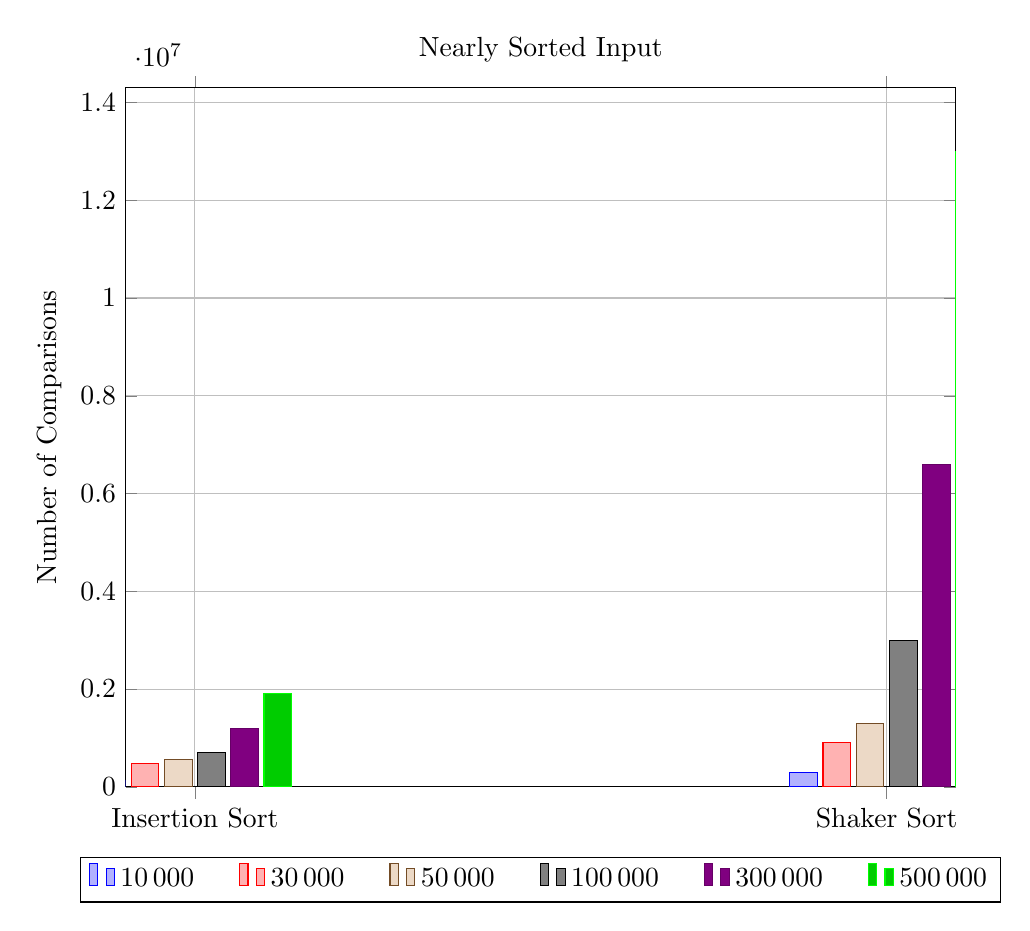
\begin{tikzpicture}
    \begin{axis}[
        width=\textwidth,
        title={Nearly Sorted Input},
        ybar,
        ymin=0,
        grid=major,
        legend style={
            at={(0.5,-0.1)}, anchor=north, legend columns=-1,
            /tikz/every even column/.append style={column sep=0.5cm}
        },
        ylabel={Number of Comparisons},
        symbolic x coords={Insertion Sort, Shaker Sort},
        xtick=data,
    ]
    \addplot coordinates {(Insertion Sort,129726) 
        (Shaker Sort,299791)};
    \addplot coordinates {(Insertion Sort,486366) 
        (Shaker Sort,899791)};
    \addplot coordinates {(Insertion Sort,560354) 
        (Shaker Sort,1299845)};
    \addplot coordinates {(Insertion Sort,706102) 
        (Shaker Sort,2999791)};
    \addplot coordinates {(Insertion Sort,1188582) 
        (Shaker Sort,6599891)};
    \addplot coordinates {(Insertion Sort,1905186) 
        (Shaker Sort,12999845)};
    \legend{10\,000, 30\,000, 50\,000, 100\,000, 300\,000, 500\,000}
    \end{axis}
\end{tikzpicture}
\caption{Kết quả thực nghiệm với đầu vào có thứ tự gần được sắp xếp (Nhóm 2)}
\end{figure}

\begin{figure}[H]
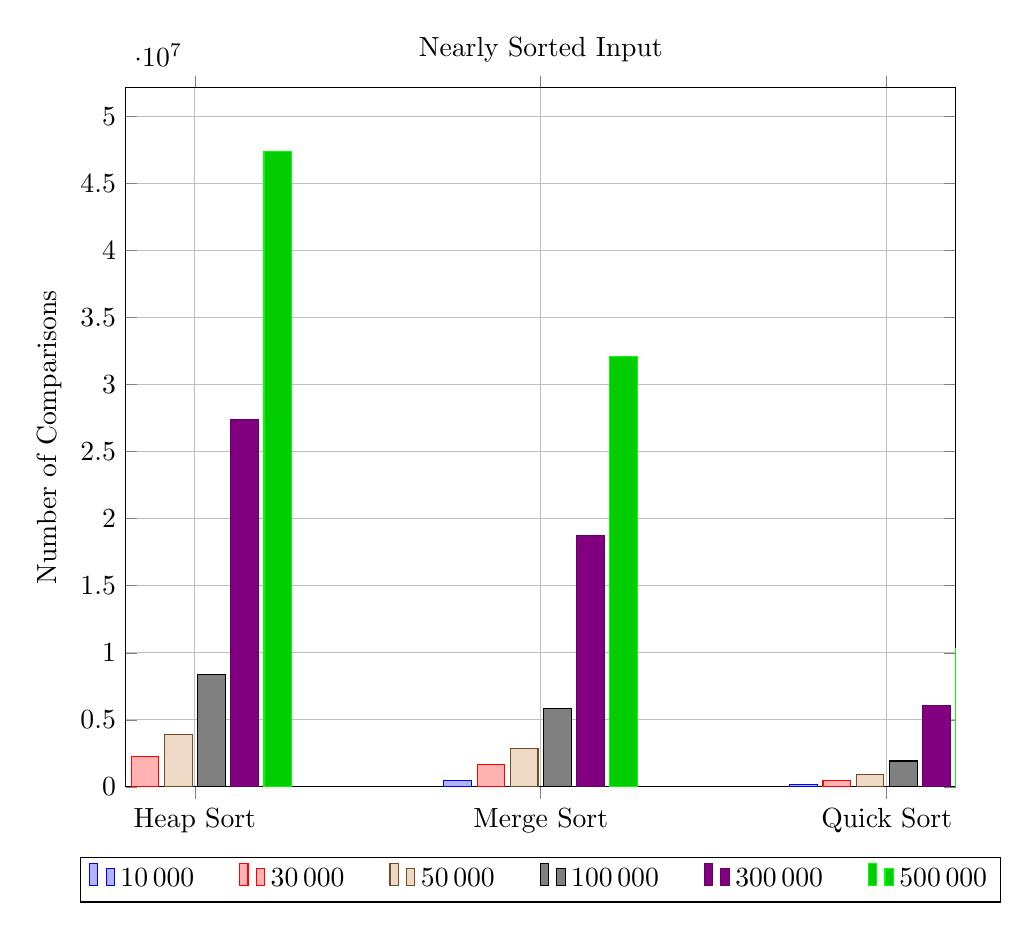
\begin{tikzpicture}
    \begin{axis}[
        width=\textwidth,
        title={Nearly Sorted Input},
        ybar,
        ymin=0,
        grid=major,
        legend style={
            at={(0.5,-0.1)}, anchor=north, legend columns=-1,
            /tikz/every even column/.append style={column sep=0.5cm}
        },
        ylabel={Number of Comparisons},
        symbolic x coords={Heap Sort, Merge Sort, Quick Sort},
        xtick=data,
    ]
    \addplot coordinates {(Heap Sort,669904) 
        (Merge Sort,503802) (Quick Sort,154995)};
    \addplot coordinates {(Heap Sort,2236774) 
        (Merge Sort,1637853) (Quick Sort,501973)};
    \addplot coordinates {(Heap Sort,3925280) 
        (Merge Sort,2845326) (Quick Sort,913890)};
    \addplot coordinates {(Heap Sort,8364715) 
        (Merge Sort,5851166) (Quick Sort,1927723)};
    \addplot coordinates {(Heap Sort,27413296) 
        (Merge Sort,18733795) (Quick Sort,6058264)};
    \addplot coordinates {(Heap Sort,47405047) 
        (Merge Sort,32137705) (Quick Sort,10310769)};
    \legend{10\,000, 30\,000, 50\,000, 100\,000, 300\,000, 500\,000}
    \end{axis}
\end{tikzpicture}
\caption{Kết quả thực nghiệm với đầu vào có thứ tự gần được sắp xếp (Nhóm 3)}
\end{figure}

\begin{figure}[H]
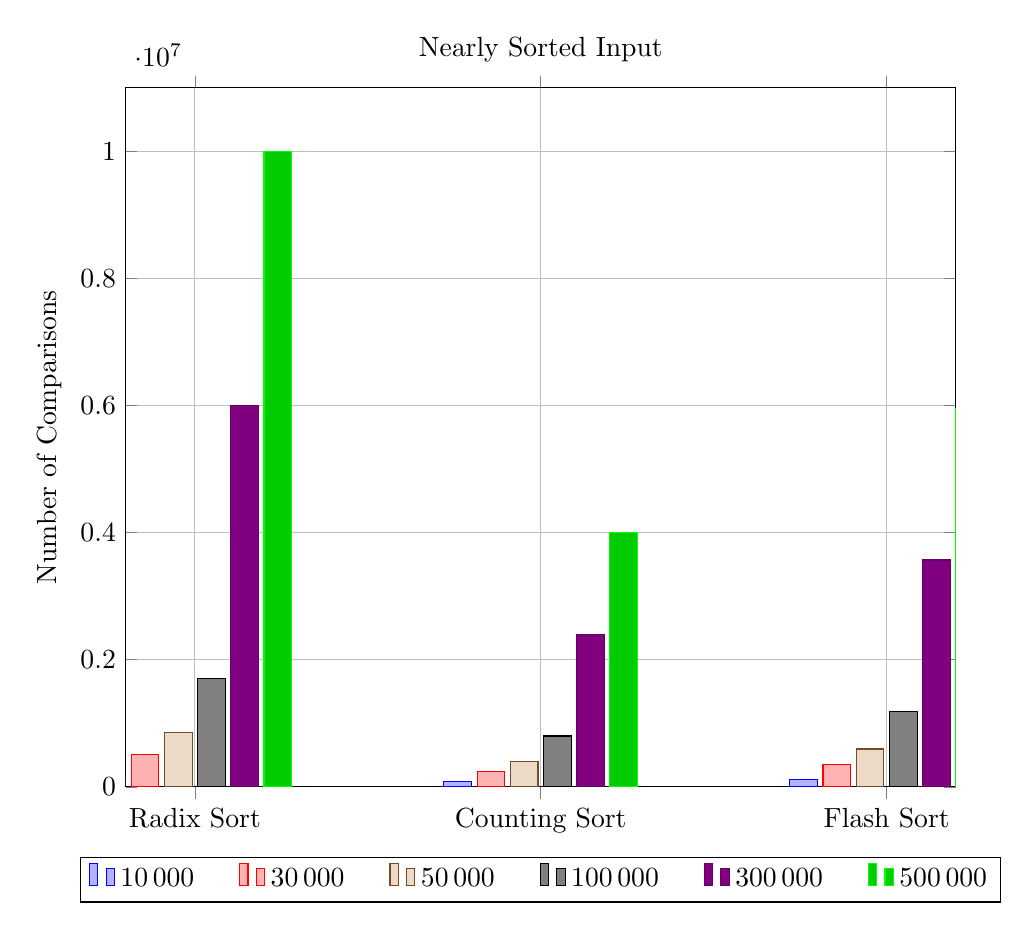
\begin{tikzpicture}
    \begin{axis}[
        width=\textwidth,
        title={Nearly Sorted Input},
        ybar,
        ymin=0,
        grid=major,
        legend style={
            at={(0.5,-0.1)}, anchor=north, legend columns=-1,
            /tikz/every even column/.append style={column sep=0.5cm}
        },
        ylabel={Number of Comparisons},
        symbolic x coords={Radix Sort, Counting Sort, Flash Sort},
        xtick=data,
    ]
    \addplot coordinates {(Radix Sort,140056) 
        (Counting Sort,80001) (Flash Sort,118969)};
    \addplot coordinates {(Radix Sort,510070) 
        (Counting Sort,240001) (Flash Sort,356969)};
    \addplot coordinates {(Radix Sort,850070) 
        (Counting Sort,400001) (Flash Sort,594969)};
    \addplot coordinates {(Radix Sort,1700070) 
        (Counting Sort,800001) (Flash Sort,1189967)};
    \addplot coordinates {(Radix Sort,6000084) 
        (Counting Sort,2400001) (Flash Sort,3569970)};
    \addplot coordinates {(Radix Sort,10000084) 
        (Counting Sort,4000001) (Flash Sort,5949970)};
    \legend{10\,000, 30\,000, 50\,000, 100\,000, 300\,000, 500\,000}
    \end{axis}
\end{tikzpicture}
\caption{Kết quả thực nghiệm với đầu vào có thứ tự gần được sắp xếp (Nhóm 4)}
\end{figure}

\begin{itemize}[label=$\circ$]
    \item Có thể nhận xét rằng số phép so sánh giữa các thuật toán sắp 
    xếp thay đổi đáng kể tùy thuộc vào độ phức tạp về thời gian và khả 
    năng tối ưu hóa đối với mảng đã có trật tự. Nhóm các thuật toán có 
    số phép so sánh lớn nhất bao gồm Selection Sort, Shell Sort, và 
    Bubble Sort do có độ phức tạp trung bình là $O\left(n^2\right)$ và 
    không tận dụng được tính chất mảng gần như đã sắp xếp. Trong đó, cả 
    ba thuật toán này đều có số phép so sánh cao nhất, đặc biệt khi kích 
    thước mảng tăng lên 300000 và 500000, với cột biểu đồ vượt trội so với 
    các thuật toán khác. Insertion Sort, nhờ khả năng tối ưu hóa tốt cho 
    các mảng đã gần được sắp xếp hoàn chỉnh, thực hiện ít phép so sánh 
    hơn đáng kể, trong khi Shaker Sort (một biến thể của Bubble Sort) cũng 
    cho thấy hiệu năng cải thiện nhưng vẫn kém hiệu quả hơn Insertion Sort. 
	\item Đối với các thuật toán có độ phức tạp trung bình là $O\left(n\log{n}\right)$ 
    về thời gian, Heap Sort thực hiện nhiều phép so sánh hơn so với Merge 
    Sort và Quick Sort. Trong đó, Quick Sort tỏ ra vượt trội hơn Merge 
    Sort nhờ khả năng tận dụng tốt tính chất của mảng gần như được sắp xếp. 
	\item Cuối cùng, nhóm thuật toán có số phép so sánh thấp nhất bao 
    gồm Radix Sort, Counting Sort và Flash Sort, nhờ đặc điểm không phụ 
    thuộc vào số phép so sánh. Nhóm này không chỉ có số phép so sánh thấp 
    nhất mà còn duy trì hiệu năng ổn định ngay cả khi kích thước mảng tăng 
    cao. Đặc biệt, Counting Sort có số phép so sánh nhỏ nhất với tất cả 
    kích thước đầu vào trong mảng có thứ tự gần được sắp xếp hoàn chỉnh.
\end{itemize}

$\bullet$ \textbf{Với đầu vào có thứ tự đã được sắp xếp}

\begin{figure}[H]
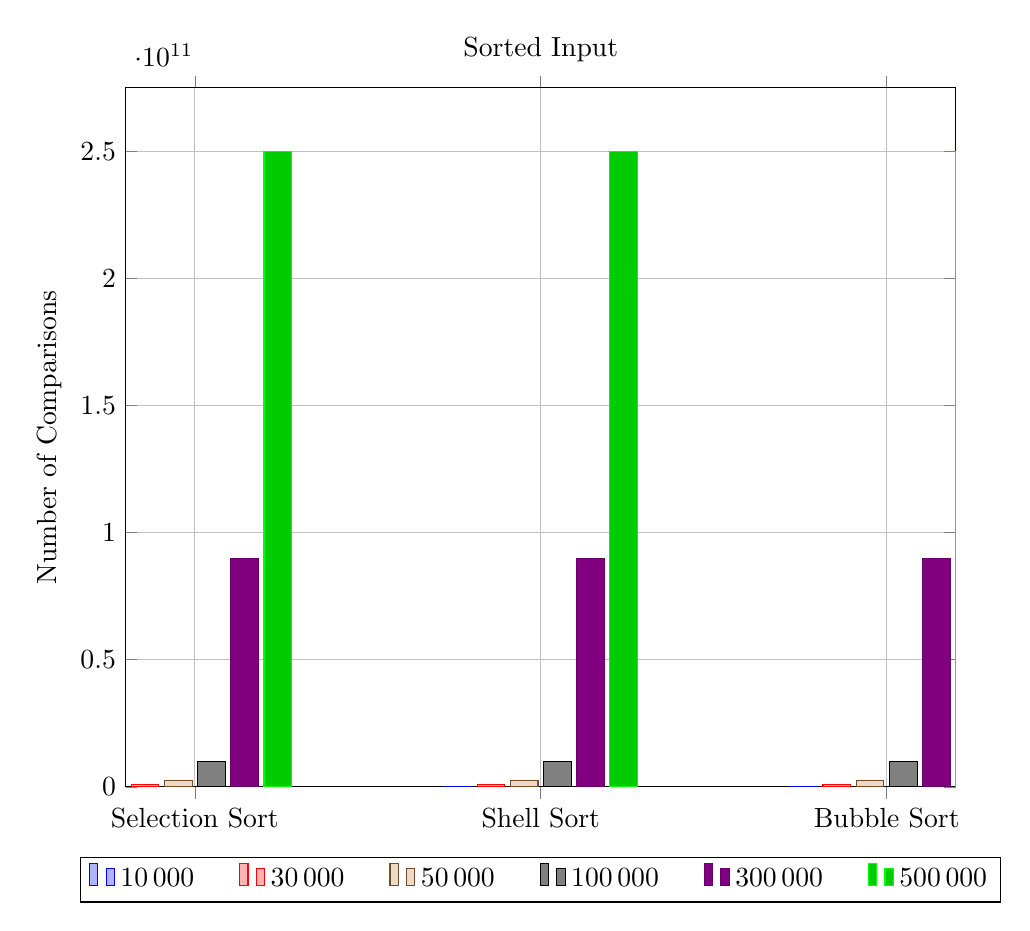
\begin{tikzpicture}
    \begin{axis}[
        width=\textwidth,
        title={Sorted Input},
        ybar,
        ymin=0,
        grid=major,
        legend style={
            at={(0.5,-0.1)}, anchor=north, legend columns=-1,
            /tikz/every even column/.append style={column sep=0.5cm}
        },
        ylabel={Number of Comparisons},
        symbolic x coords={Selection Sort, Shell Sort, Bubble Sort},
        xtick=data,
    ]
    \addplot coordinates {(Selection Sort,100009999) 
        (Shell Sort,100009999) (Bubble Sort,100009999)};
    \addplot coordinates {(Selection Sort,900029999) 
        (Shell Sort,900029999) (Bubble Sort,900029999)};
    \addplot coordinates {(Selection Sort,2500049999) 
        (Shell Sort,2500049999) (Bubble Sort,2500049999)};
    \addplot coordinates {(Selection Sort,10000099999) 
        (Shell Sort,10000099999) (Bubble Sort,10000099999)};
    \addplot coordinates {(Selection Sort,90000299999) 
        (Shell Sort,90000299999) (Bubble Sort,90000299999)};
    \addplot coordinates {(Selection Sort,250000499999) 
        (Shell Sort,250000499999) (Bubble Sort,250000499999)};
    \legend{10\,000, 30\,000, 50\,000, 100\,000, 300\,000, 500\,000}
    \end{axis}
\end{tikzpicture}
\caption{Kết quả thực nghiệm với đầu vào có thứ tự đã được sắp xếp (Nhóm 1)}
\end{figure}

\begin{figure}[H]
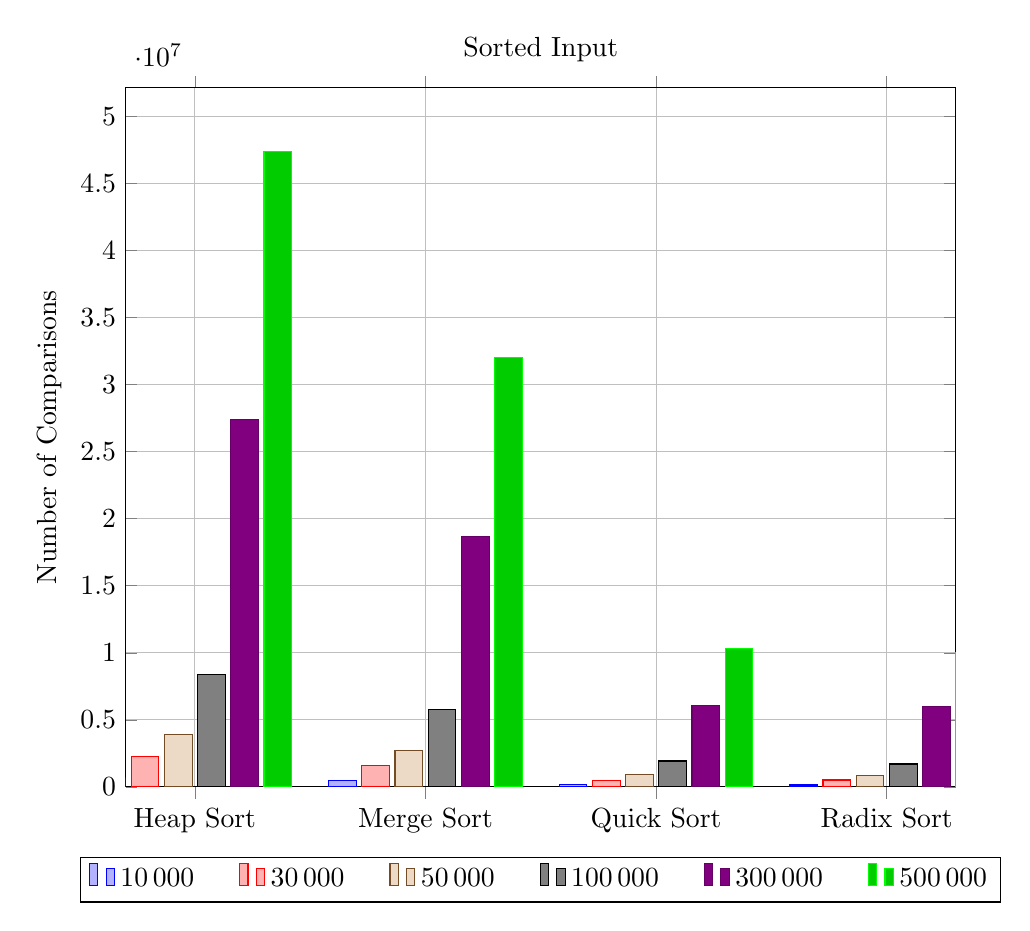
\begin{tikzpicture}
    \begin{axis}[
        width=\textwidth,
        title={Sorted Input},
        ybar,
        ymin=0,
        grid=major,
        legend style={
            at={(0.5,-0.1)}, anchor=north, legend columns=-1,
            /tikz/every even column/.append style={column sep=0.5cm}
        },
        ylabel={Number of Comparisons},
        symbolic x coords={Heap Sort, Merge Sort, Quick Sort, Radix Sort},
        xtick=data,
    ]
    \addplot coordinates {(Heap Sort,670329) (Merge Sort,475242) 
        (Quick Sort,154959) (Radix Sort,140056)};
    \addplot coordinates {(Heap Sort,2236648) (Merge Sort,1559914) 
        (Quick Sort,501929) (Radix Sort,510070)};
    \addplot coordinates {(Heap Sort,3925351) (Merge Sort,2722826) 
        (Quick Sort,913850) (Radix Sort,850070)};
    \addplot coordinates {(Heap Sort,8365080) (Merge Sort,5745658) 
        (Quick Sort,1927691) (Radix Sort,1700070)};
    \addplot coordinates {(Heap Sort,27413230) (Merge Sort,18645946) 
        (Quick Sort,6058228) (Radix Sort,6000084)};
    \addplot coordinates {(Heap Sort,47404886) (Merge Sort,32017850) 
        (Quick Sort,10310733) (Radix Sort,10000084)};
    \legend{10\,000, 30\,000, 50\,000, 100\,000, 300\,000, 500\,000}
    \end{axis}
\end{tikzpicture}
\caption{Kết quả thực nghiệm với đầu vào có thứ tự đã được sắp xếp (Nhóm 2)}
\end{figure}

\begin{figure}[H]
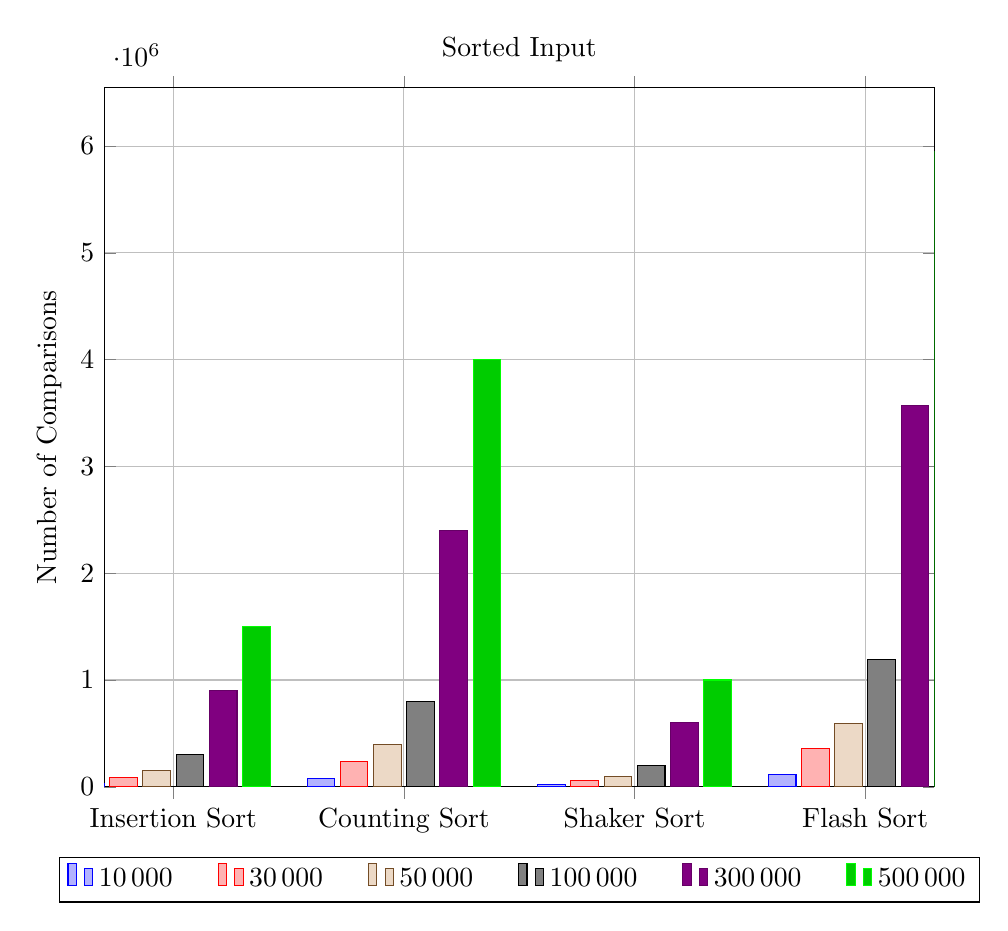
\begin{tikzpicture}
    \begin{axis}[
        width=\textwidth,
        title={Sorted Input},
        ybar,
        ymin=0,
        grid=major,
        legend style={
            at={(0.5,-0.1)}, anchor=north, legend columns=-1,
            /tikz/every even column/.append style={column sep=0.5cm}
        },
        ylabel={Number of Comparisons},
        symbolic x coords={Insertion Sort, Counting Sort, Shaker Sort, Flash Sort},
        xtick=data,
    ]
    \addplot coordinates {(Insertion Sort,29998) 
        (Counting Sort,80001) (Shaker Sort,20001) (Flash Sort,118993)};
    \addplot coordinates {(Insertion Sort,89998) 
        (Counting Sort,240001) (Shaker Sort,60001) (Flash Sort,356993)};
    \addplot coordinates {(Insertion Sort,149998) 
        (Counting Sort,400001) (Shaker Sort,100001) (Flash Sort,594993)};
    \addplot coordinates {(Insertion Sort,299998) 
        (Counting Sort,800001) (Shaker Sort,200001) (Flash Sort,1189993)};
    \addplot coordinates {(Insertion Sort,899998) 
        (Counting Sort,2400001) (Shaker Sort,600001) (Flash Sort,3569993)};
    \addplot coordinates {(Insertion Sort,1499998) 
        (Counting Sort,4000001) (Shaker Sort,1000001) (Flash Sort,5949993)};
    \legend{10\,000, 30\,000, 50\,000, 100\,000, 300\,000, 500\,000}
    \end{axis}
\end{tikzpicture}
\caption{Kết quả thực nghiệm với đầu vào có thứ tự đã được sắp xếp (Nhóm 3)}
\end{figure}

\begin{itemize}[label=$\circ$]
    \item Selection Sort, Shell Sort và Bubble Sort thực hiện một lượng 
    rất lớn số phép so sánh, đặc biệt là khi kích thước đầu vào lớn. Đó 
    là do các thuật toán này không có cách nào để “nhận ra” mảng đã được 
    sắp xếp xong nên liên tục thực hiện những phép so sánh vô nghĩa.
    \item Thuật toán Shaker Sort có số phép so sánh nhỏ nhất trong bảng 
    số liệu. Là một phiên bản cải tiến của Bubble Sort nên khi mảng đã 
    được sắp xếp sẵn, Shaker Sort chỉ cần duyệt qua mảng để xác nhận 
    rằng nó đã sắp xếp đúng, dẫn đến số phép so sánh rất thấp. Bên cạnh 
    đó, Insertion Sort cũng có số phép so sánh ít trong trường hợp mảng 
    đã được sắp xếp sẵn vì mỗi phần tử chỉ cần kiểm tra một lần với phần 
    tử liền trước để đảm bảo vị trí đúng mà không cần thực hiện thêm phép 
    so sánh nào khác.
\end{itemize}

\pagebreak

$\bullet$ \textbf{Với đầu vào có thứ tự được sắp xếp ngược}

\begin{figure}[H]
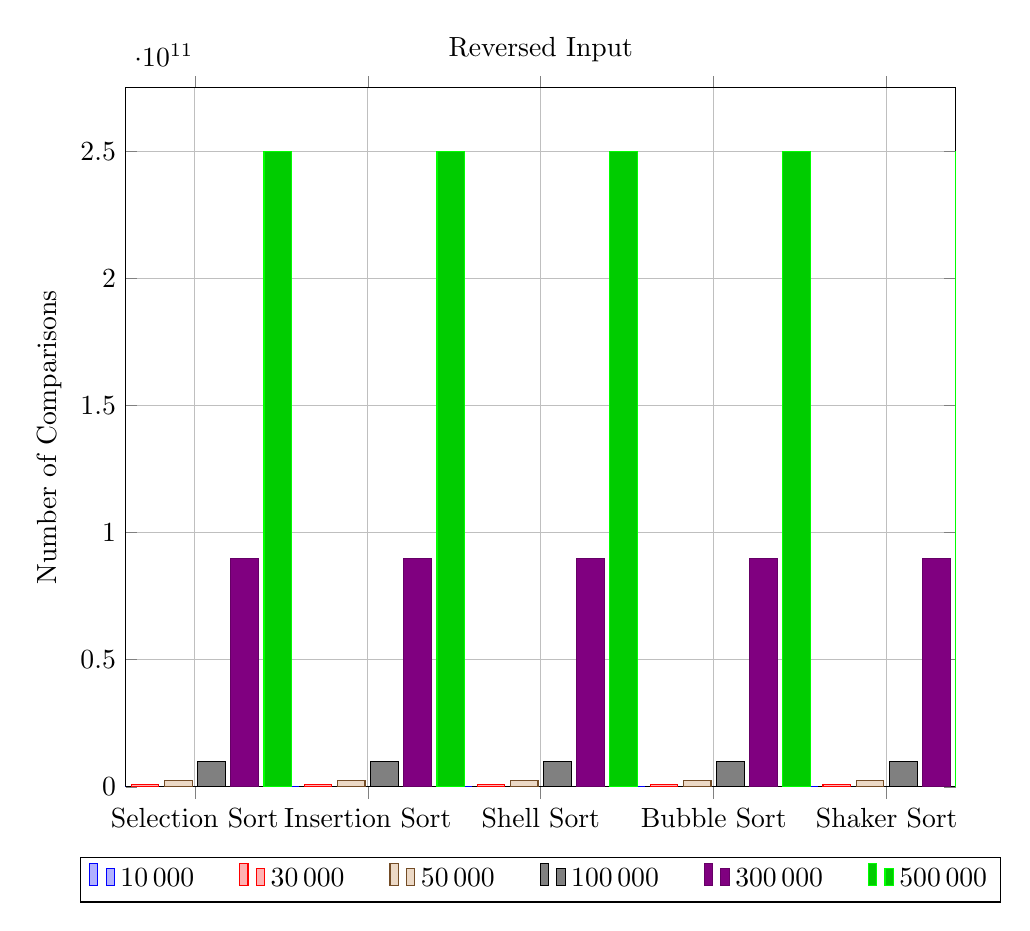
\begin{tikzpicture}
    \begin{axis}[
        width=\textwidth,
        title={Reversed Input},
        ybar,
        ymin=0,
        grid=major,
        legend style={
            at={(0.5,-0.1)}, anchor=north, legend columns=-1,
            /tikz/every even column/.append style={column sep=0.5cm}
        },
        ylabel={Number of Comparisons},
        symbolic x coords={Selection Sort, Insertion Sort, Shell Sort, Bubble Sort, Shaker Sort},
        xtick=data,
    ]
    \addplot coordinates {(Selection Sort,100009999) (Insertion Sort,100009999)
        (Shell Sort,100009999) (Bubble Sort,100009999) (Shaker Sort,100010001)};
    \addplot coordinates {(Selection Sort,900029999) (Insertion Sort,900029999)
        (Shell Sort,900029999) (Bubble Sort,900029999) (Shaker Sort,900030001)};
    \addplot coordinates {(Selection Sort,2500049999) (Insertion Sort,2500049999)
        (Shell Sort,2500049999) (Bubble Sort,2500049999) (Shaker Sort,2500050001)};
    \addplot coordinates {(Selection Sort,10000099999) (Insertion Sort,10000099999)
        (Shell Sort,10000099999) (Bubble Sort,10000099999) (Shaker Sort,10000100001)};
    \addplot coordinates {(Selection Sort,90000299999) (Insertion Sort,90000299999)
        (Shell Sort,90000299999) (Bubble Sort,90000299999) (Shaker Sort,90000300001)};
    \addplot coordinates {(Selection Sort,250000499999) (Insertion Sort,250000499999)
        (Shell Sort,250000499999) (Bubble Sort,250000499999) (Shaker Sort,250000500001)};
    \legend{10\,000, 30\,000, 50\,000, 100\,000, 300\,000, 500\,000}
    \end{axis}
\end{tikzpicture}
\caption{Kết quả thực nghiệm với đầu vào có thứ tự được sắp xếp ngược (Nhóm 1)}
\end{figure}

\begin{figure}[H]
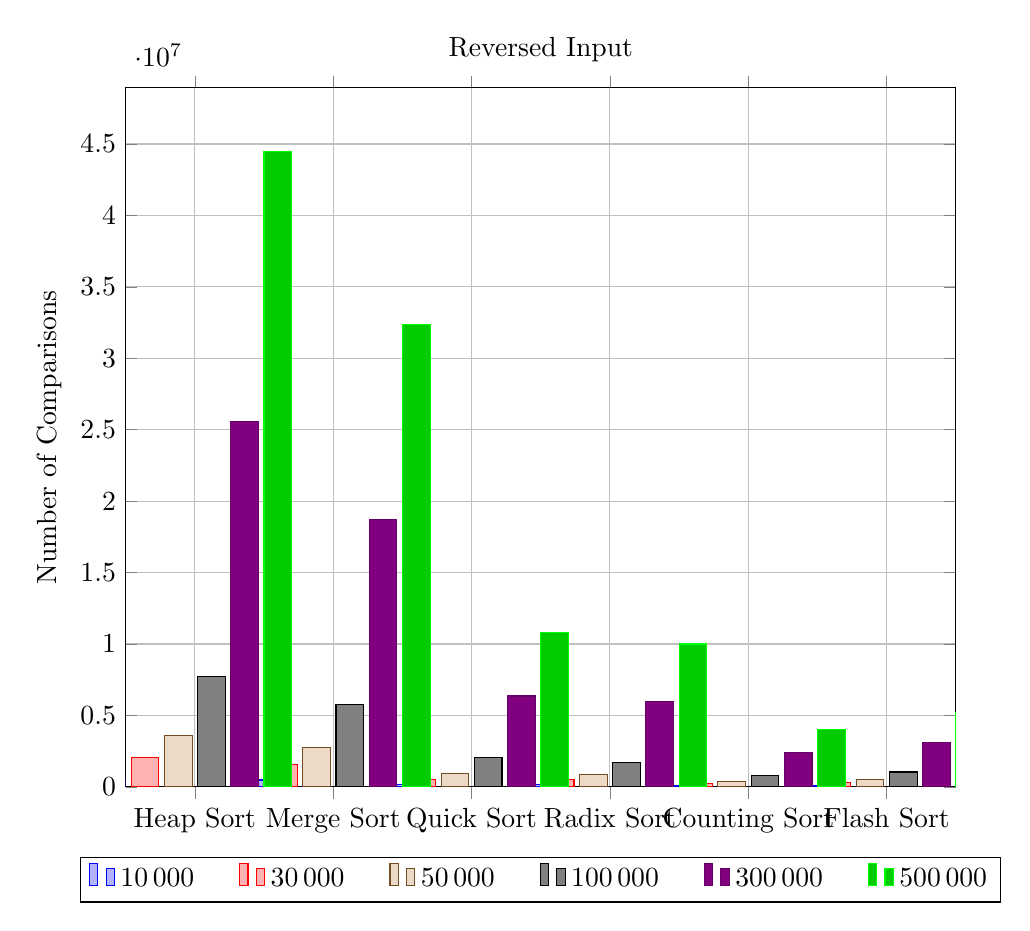
\begin{tikzpicture}
    \begin{axis}[
        width=\textwidth,
        title={Reversed Input},
        ybar,
        ymin=0,
        grid=major,
        legend style={
            at={(0.5,-0.1)}, anchor=north, legend columns=-1,
            /tikz/every even column/.append style={column sep=0.5cm}
        },
        ylabel={Number of Comparisons},
        symbolic x coords={Heap Sort, Merge Sort, Quick Sort, Radix Sort, Counting Sort, Flash Sort},
        xtick=data,
    ]
    \addplot coordinates {(Heap Sort,606771) (Merge Sort,476441) (Quick Sort,164975)
        (Radix Sort,140056) (Counting Sort,80001) (Flash Sort,103751)};
    \addplot coordinates {(Heap Sort,2063324) (Merge Sort,1573465) (Quick Sort,531939)
        (Radix Sort,510070) (Counting Sort,240001) (Flash Sort,311251)};
    \addplot coordinates {(Heap Sort,3612724) (Merge Sort,2733945) (Quick Sort,963861)
        (Radix Sort,850070) (Counting Sort,400001) (Flash Sort,518751)};
    \addplot coordinates {(Heap Sort,7718943) (Merge Sort,5767897) (Quick Sort,2027703)
        (Radix Sort,1700070) (Counting Sort,800001) (Flash Sort,1037501)};
    \addplot coordinates {(Heap Sort,25569379) (Merge Sort,18708313) (Quick Sort,6358249)
        (Radix Sort,6000084) (Counting Sort,2400001) (Flash Sort,3112501)};
    \addplot coordinates {(Heap Sort,44483348) (Merge Sort,32336409) (Quick Sort,10810747)
        (Radix Sort,10000084) (Counting Sort,4000001) (Flash Sort,5187501)};
    \legend{10\,000, 30\,000, 50\,000, 100\,000, 300\,000, 500\,000}
    \end{axis}
\end{tikzpicture}
\caption{Kết quả thực nghiệm với đầu vào có thứ tự được sắp xếp ngược (Nhóm 2)}
\end{figure}

\begin{itemize}[label=$\circ$]
    \item Selection Sort, Insertion Sort, Shell Sort, Bubble Sort và 
    Shaker Sort đều có số phép so sánh rất lớn trong trường hợp mảng được 
    sắp xếp ngược vì đây là trường hợp xấu nhất - mọi phần tử đều nằm sai 
    vị trí. Khi đó, các thuật toán này phải kiểm tra và điều chỉnh vị trí 
    của từng phần tử thông qua nhiều lần duyệt hoặc so sánh cặp.
    \item Counting Sort và Flash Sort có số phép so sánh khá ít trong 
    trường hợp này. Trong khi Counting Sort chỉ dựa trên việc đếm số lượng 
    phần tử trong các giá trị hoặc phạm vi thì Flash Sort sử dụng cách 
    phân chia mảng thành các nhóm dựa trên giá trị. Cả hai thuật toán này 
    đều hạn chế so sánh trực tiếp giữa các phần tử nên dù cho mảng có sắp 
    xếp ngược vẫn không ảnh hưởng quá nhiều.
\end{itemize}

\pagebreak

$\blacktriangleright$ \textbf{Kết luận:}
\\\\
Dựa trên các kết quả thực nghiệm, hiệu suất của các thuật toán sắp xếp 
thay đổi đáng kể tùy thuộc vào kiểu thứ tự mảng đầu vào và kích thước 
mảng. \textbf{Counting Sort} và \textbf{Radix Sort} là những thuật toán nhanh nhất 
trong các trường hợp dữ liệu phù hợp, với độ phức tạp trung bình và tốt nhất 
lần lượt là $O\left(n+k\right)$ và $O\left(d\times\left(n+k\right)\right)$. 
Chúng hoạt động hiệu quả trên các mảng lớn có giá trị nguyên và phạm vi 
giá trị nhỏ hoặc cố định. Tuy nhiên, khi $k$ (phạm vi giá trị) hoặc $d$ 
(số chữ số lớn nhất) tăng, hiệu suất của chúng có thể bị ảnh hưởng. 
Ngược lại, \textbf{Flash Sort} đạt được hiệu suất $O\left(n\right)$ trong 
trường hợp tốt nhất và trung bình, vượt trội trên các mảng có kích thước 
lớn và giá trị phân bố đều (và là số nguyên).
\\\\
Xét nhóm thuật toán có độ phức tạp trung bình là $O\left(n\log{n}\right)$ 
thì ta có thể thấy hiệu suất ổn định với mọi kiểu dữ liệu đầu vào (ngẫu 
nhiên, đảo ngược, ...) của \textbf{Heap Sort} và \textbf{Merge Sort}. Trong khi đó, 
\textbf{Quick Sort} vượt trội với thời gian ngắn nhất do chọn $pivot$ hợp 
lí (khi chọn $pivot$ tệ sẽ khiến độ phức tạp của Quick Sort lên đến 
$O\left(n^2\right)$).
\\\\
Nhóm thuật toán đơn giản nhất (độ phức tạp thời gian $O\left(n^2\right)$) 
chi phí thực thi khá thấp với số lượng phần tử nhỏ $(n < 10,000)$. Với 
kiểu dữ liệu gần như được sắp xếp hay đã sắp xếp thì \textbf{Shaker Sort} và 
\textbf{Insertion Sort} đã vượt trội hẳn với các thuật toán còn lại trong 
nhóm này với độ phức tạp $O\left(n\right)$ (trường hợp tốt nhất của 2 
thuật toán này). Còn với những thuật toán còn lại như \textbf{Selection Sort} 
và \textbf{Bubble Sort} luôn chạy với độ phức tạp là $O\left(n^2\right)$ 
trong mọi trường hợp, \textbf{Shell Sort} có thể cải thiện thời gian thực 
thi nếu chọn $gap$ tốt (lúc này độ phức tạp sẽ là $O\left(n\log{n}\right)$).
\\\\
Kích thước mảng cũng ảnh hưởng lớn đến hiệu suất của các thuật toán. Với 
các mảng nhỏ (dưới 10,000 phần tử), các thuật toán đơn giản như 
\textbf{Selection Sort}, \textbf{Bubble Sort}, \textbf{Shaker Sort}, 
\textbf{Insertion Sort} và \textbf{Shell Sort} hoạt động tốt nhờ chi phí 
thấp và khả năng tối ưu hóa trên mảng nhỏ. Với mảng trung bình (10,000 đến 
100,000 phần tử), các thuật toán có độ phức tạp thời gian là 
$O\left(n\log{n}\right)$ như \textbf{Quick Sort}, \textbf{Heap Sort} và 
\textbf{Merge Sort} bắt đầu thể hiện ưu thế. Đối với mảng lớn (trên 
100,000 phần tử), \textbf{Counting Sort}, \textbf{Radix Sort} và 
\textbf{Flash Sort} là những sự lựa chọn hàng đầu nếu dữ liệu đầu vào 
phù hợp như đã nói ở trên.

\pagebreak

Tính ổn định của thuật toán cũng là một yếu tố quan trọng trong một số 
bài toán. \textbf{Bubble Sort}, \textbf{Shaker Sort}, \textbf{Insertion 
Sort}, \textbf{Merge Sort}, \textbf{Counting Sort} và \textbf{Radix Sort} 
là các thuật toán ổn định, giữ nguyên thứ tự của các phần tử bằng nhau 
trong mảng đầu vào. Điều này rất hữu ích trong các bài toán yêu cầu sắp 
xếp theo nhiều tiêu chí. Ngược lại, \textbf{Selection Sort}, \textbf{Shell 
Sort}, \textbf{Heap Sort}, \textbf{Quick Sort} và \textbf{Flash Sort} 
không đảm bảo tính ổn định, do cách hoán đổi các phần tử. 
\\\\
Tóm lại, \textbf{Counting Sort}, \textbf{Radix Sort} và \textbf{Flash Sort} 
vượt trội về tốc độ trong các trường hợp phù hợp, trong khi \textbf{Counting 
Sort}, \textbf{Radix Sort} và \textbf{Flash Sort} là những thuật toán toàn 
diện và ổn định về hiệu suất trên nhiều loại thứ tự mảng cũng như kích 
thước mảng đầu vào. \textbf{Shaker Sort} và \textbf{Insertion Sort} là lựa 
chọn tốt cho các mảng nhỏ hoặc đã được sắp xếp hoặc gần như được sắp xếp 
hoàn chỉnh. Các thuật toán như \textbf{Selection Sort}, \textbf{Bubble Sort} 
hay \textbf{Shell Sort} tuy dễ triển khai nhưng không hiệu quả với mảng lớn. 
Những nhận xét tổng quát cho toàn bộ dựa trên các kiểu thứ tự và kích thước 
mảng đầu vào nói trên đã giúp làm rõ sự khác biệt giữa các thuật toán và 
cung cấp cái nhìn sâu sắc về cách chọn thuật toán phù hợp cho từng bài toán 
cụ thể.